% template by Natalia Chernov for the University of Oldenburg

\documentclass[xcolor=table,9pt,aspectratio=169]{beamer}

\usepackage[utf8]{inputenc}

\usepackage{anyfontsize}
\usepackage[english,ngerman]{babel}
\usepackage[autostyle]{csquotes}
\usepackage{datetime}
\usepackage{helvet}
   \renewcommand{\familydefault}{\sfdefault}
\usepackage{lipsum}
\usepackage{lmodern}
\usepackage{multicol}
\usepackage{smartdiagram}
\usepackage{tikz}

\definecolor{uolblue}{RGB}{0,62,107}

\definecolor{blue1}{RGB}{0,78,159}
\definecolor{blue2}{RGB}{0,171,217}
\definecolor{blue3}{RGB}{91,197,242}
\definecolor{blue4}{RGB}{161,217,248}

\definecolor{green1}{RGB}{0,120,120}
\definecolor{green2}{RGB}{0,168,121}
\definecolor{green3}{RGB}{148,193,28}
\definecolor{green4}{RGB}{199,211,0}

\definecolor{orange1}{RGB}{213,59,10}
\definecolor{orange2}{RGB}{238,113,0}
\definecolor{orange3}{RGB}{243,145,0}
\definecolor{orange4}{RGB}{253,195,0}

\definecolor{gr}{RGB}{191,191,191}

\setbeameroption{hide notes}
% \setbeameroption{show only notes}
% \setbeameroption{show notes on second screen=right}

\setbeamertemplate{frametitle}{\color{uolblue}\fontsize{12}{20}\selectfont{\insertframetitle}}

\pgfdeclareimage[width=0.145\paperwidth]{logo}{figures/slides_logo_uol_negative}
\pgfdeclareimage[width=0.072\paperwidth]{logo_small}{figures/slides_logo_uol_negative}

\defbeamertemplate*{background canvas}{default_page}
{%
\begin{tikzpicture}
   \useasboundingbox (0,0) rectangle (\the\paperwidth,\the\paperheight);
   \filldraw[fill=uolblue,fill opacity=1,draw=none] (0,0) rectangle (0.119\paperwidth,\the\paperheight);
   \filldraw[fill=blue2,fill opacity=1,draw=none] (0.119\paperwidth,0) -- (0.119\paperwidth,0.565\paperheight) arc (117.2:180:0.6\paperwidth) -- cycle;
   \pgftext[at=\pgfpoint{10}{\the\paperheight-11.5},left,top]{\pgfsetfillopacity{1}\pgfuseimage{logo_small}};
\end{tikzpicture}
}
\defbeamertemplate*{background canvas}{titlepage_image}
{
\begin{tikzpicture}
   \useasboundingbox (0,0) rectangle (\the\paperwidth,\the\paperheight);
   \filldraw[fill=uolblue,fill opacity=1,draw=none] (0,0) rectangle (\the\paperwidth,\the\paperheight);
   \filldraw[fill=blue2,fill opacity=1,draw=none] (\the\paperwidth,0) -- (\the\paperwidth,0.66\paperheight) arc (90:180:0.6\paperwidth) -- cycle;
   \pgftext[at=\pgfpoint{14}{\the\paperheight-17.5},left,top]{\pgfsetfillopacity{1}\pgfuseimage{logo}};
\end{tikzpicture}
}
\BeforeBeginEnvironment{frame}{%
   \setbeamertemplate{background canvas}[default_page]%
}
\makeatletter
\define@key{beamerframe}{titlepage_image}[true]{%
   \setbeamercovered{invisible}%
   \setbeamertemplate{background canvas}[titlepage_image]%
}
\makeatother%

\setbeamertemplate{footline}
{
   \leavevmode
   \hbox{
   \hspace*{.025\paperwidth}\begin{beamercolorbox}[wd=.094\paperwidth,ht=2.25ex,dp=1ex,left]{}
   ~

   \vspace*{.042\paperheight}
      \fontsize{4.4}{5.9}\selectfont\color{white}\textbf{Folie \insertframenumber}\newline\insertdate
   \vspace*{.026\paperheight}
   \end{beamercolorbox}
   \hspace*{.05\paperwidth}\begin{beamercolorbox}
   [wd=.79\paperwidth,ht=2.25ex,dp=1ex,left]{}
   ~

   \vspace*{.042\paperheight}
      \fontsize{4.4}{5.9}\selectfont\color{black}\textbf{Empirische Studien zu Fragen der Bedarfsgerechtigkeit}\newline\color{gray}\insertauthor~--~Fakultät IV, Institut für Philosophie
   \vspace*{.026\paperheight}
   \end{beamercolorbox}
   }
   \vskip0pt
}

\setbeamerfont{title}{size={\fontsize{22}{25}}}
\setbeamerfont{subtitle}{size={\fontsize{12}{14}}}
\setbeamerfont{author}{size={\fontsize{9}{11}}}
\setbeamerfont{date}{size={\fontsize{9}{11}}}
\setbeamercolor{title}{fg=white}
\setbeamercolor{subtitle}{fg=white}
\setbeamercolor{author}{fg=white}
\setbeamercolor{date}{fg=white}
\setbeamercolor{color_Logo-Platzhalter}{fg=white,bg=gray!40}

\defbeamertemplate*{title page}{customized}[1][]
{  \vspace*{20mm}
   \hspace*{-22.5mm}
   \begin{minipage}{\textwidth}
   \usebeamerfont{title}\usebeamercolor[fg]{title}\inserttitle\par
   \bigskip
   \usebeamerfont{subtitle}\usebeamercolor[fg]{subtitle}\insertsubtitle\par
   \bigskip
   \usebeamerfont{author}\usebeamercolor[fg]{author}\insertauthor,
   \usebeamerfont{date}\usebeamercolor[fg]{date}\insertdate\par
   \end{minipage}
}
\setbeamertemplate{navigation symbols}{}
\setbeamersize{text margin left=0.17\paperwidth,text margin right=0.04\paperwidth}

\title{Empirische Studien zu Fragen\\der Bedarfsgerechtigkeit}
\subtitle{}
\author{Alexander Max Bauer}
\date{\renewcommand{\dateseparator}{.}\ddmmyyyydate\today}
\usepackage{enumitem}
\def\labelitemi{--}
\def\labelitemii{--}
\def\labelitemiii{--}

\begin{document}
{
\setbeamertemplate{footline}{}
\begin{frame}[titlepage_image]
   \maketitle
\end{frame}
}


%%%%%%%%%%%
% FOLIE 2 %
%%%%%%%%%%%
\begin{frame}{\vspace*{10mm}Gliederung}
\begin{itemize}
   \item[1] \hspace*{1em}Vorgeschichte
   \item[2] \hspace*{1em}Empirische Forschung und normative Theorie \textcolor{gray}{(Bauer und Meyerhuber 2019)}
   \item[3] \hspace*{1em}Bedarf und Bedarfsgerechtigkeit \textcolor{gray}{(Bauer 2019)}
   \item[4] \hspace*{1em}Bedarf als Referenzpunkt \textcolor{gray}{(Bauer et al. 2023a)}
   \item[5] \hspace*{1em}Bedarf und Verantwortung \textcolor{gray}{(Bauer et al. 2022, Bauer und Romann i.\,V.)}
   \item[6] \hspace*{1em}Bedarfsarten \textcolor{gray}{(Bauer et al. 2023b)}
   \item[7] \hspace*{1em}Zusammenfassung zentraler Ergebnisse \textcolor{gray}{(Bauer und Siebel i.\,V.)}
\end{itemize}
\end{frame}


%%%%%%%%%%%
% FOLIE 3 %
%%%%%%%%%%%
\begin{frame}
\begin{overlayarea}{\textwidth}{0.81\paperheight}{
   \vspace*{11mm}
   \usebeamerfont{title}\textcolor{uolblue}
   {1\hspace*{1em}Vorgeschichte}
}
\end{overlayarea}
\end{frame}


%%%%%%%%%%%
% FOLIE 4 %
%%%%%%%%%%%
\begin{frame}{\vspace*{10mm}1\hspace*{1em}Vorgeschichte}
\frame{
\includegraphics[width=0.8\linewidth]{figures/slides_email.png}}
\end{frame}


%%%%%%%%%%%
% FOLIE 5 %
%%%%%%%%%%%
\begin{frame}{\vspace*{10mm}1\hspace*{1em}Vorgeschichte}
\frame{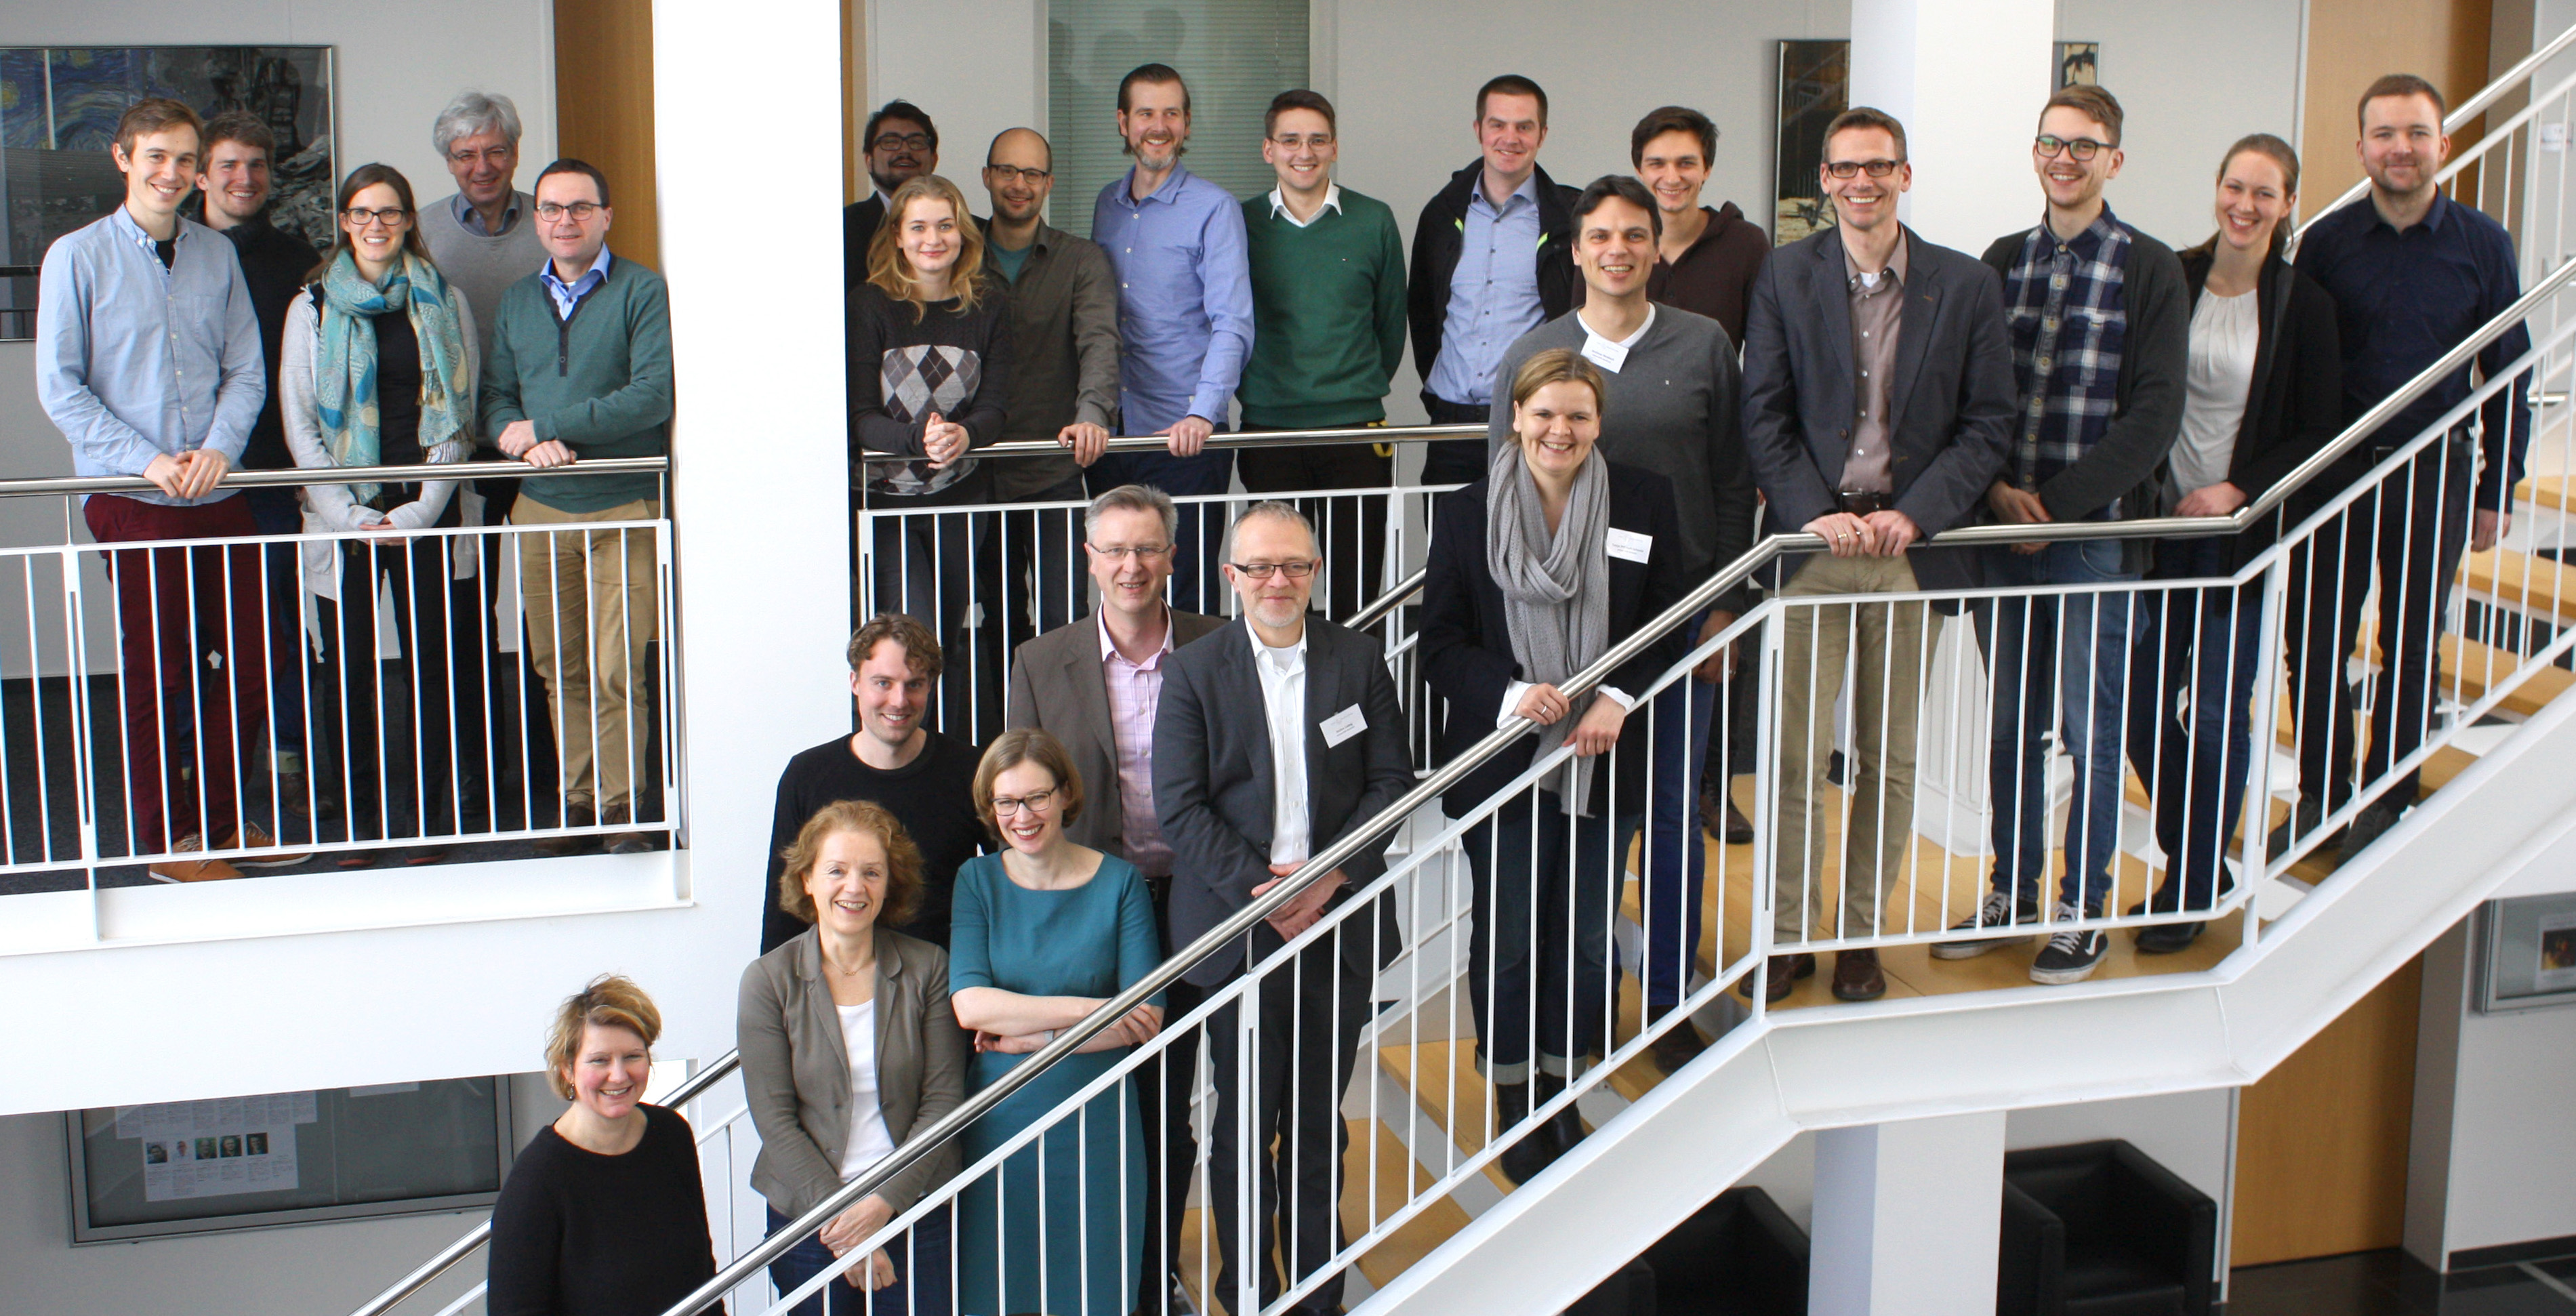
\includegraphics[width=0.8\linewidth]{figures/slides_for.jpg}}
\note{
   \begin{itemize}
      \item Hanse-Wissenschaftskolleg Delmenhorst 2017
   \end{itemize}
}
\end{frame}


%%%%%%%%%%%
% FOLIE 6 %
%%%%%%%%%%%
\begin{frame}{\vspace*{10mm}1\hspace*{1em}Vorgeschichte}
\frame{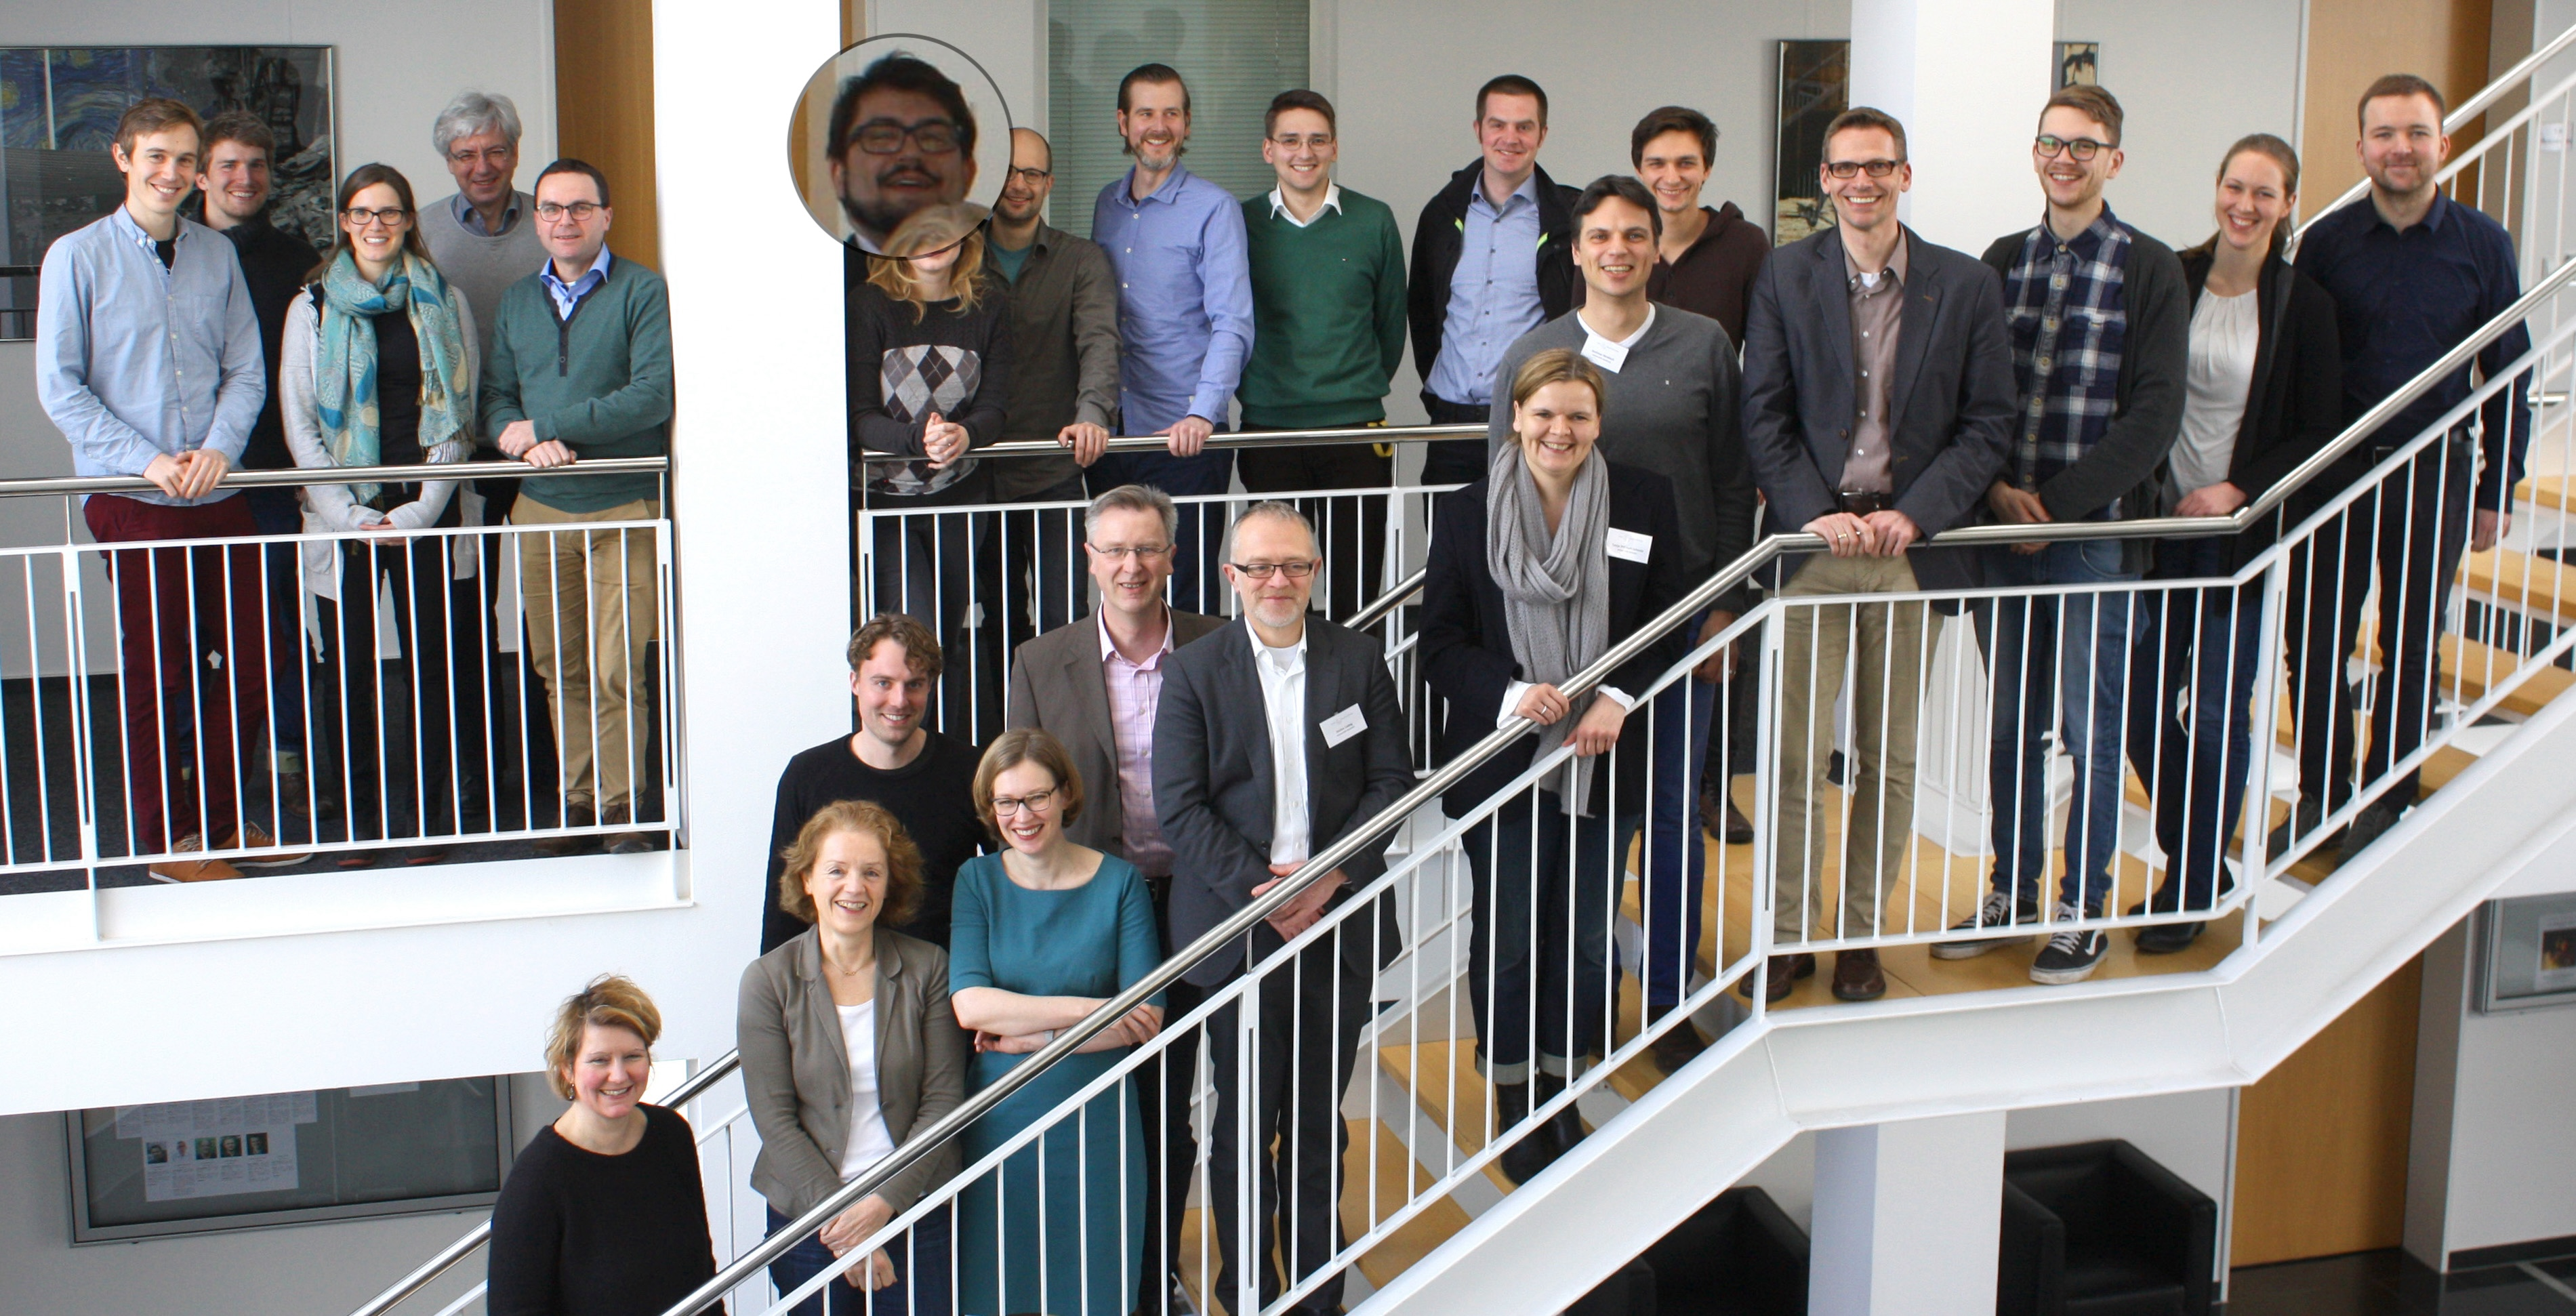
\includegraphics[width=0.8\linewidth]{figures/slides_for_close_up.jpg}}
\end{frame}


%%%%%%%%%%%
% FOLIE 7 %
%%%%%%%%%%%
\begin{frame}
\begin{overlayarea}{\textwidth}{0.81\paperheight}{
   \vspace*{11mm}
   \usebeamerfont{title}\textcolor{uolblue}
   {2\hspace*{1em}Empirische Forschung\\\hspace*{1.5em}und normative Theorie}
}
\end{overlayarea}
\end{frame}


%%%%%%%%%%%
% FOLIE 8 %
%%%%%%%%%%%
\begin{frame}{\vspace*{10mm}2\hspace*{1em}Empirische Forschung und normative Theorie}
\textbf{Verortung}\\
\medskip
\begin{itemize}
   \item Deskriptive Ethik $\in$ Experimentelle Philosophie
   \item Experimentelle Philosophie $\in$ Philosophie
\end{itemize}
\end{frame}


%%%%%%%%%%%
% FOLIE 9 %
%%%%%%%%%%%
\begin{frame}{\vspace*{10mm}2\hspace*{1em}Empirische Forschung und normative Theorie}
\begin{multicols}{2}
   \textbf{Relevanz}\\
   \medskip
   \begin{itemize}
      \item \enquote{komplementäre Angewiesenheit [\ldots] von empirischer Gerechtigkeitsforschung und normativer Gerechtigkeitstheorie} \textcolor{gray}{(Honneth 2008, S. 10)}
      \item Experimentelle Philosophie kann einen Beitrag zur Ethik leisten
      \begin{itemize}
         \item Erweiterung der Grundgesamtheit an Introspektionen, die zur Reflexion zur Verfügung stehen
         \item Falsifikation oder Verifikation empirischer Pr\"amissen
         \item Ex-ante- und Ex-post Evaluation der Implementation
      \end{itemize}
   \end{itemize}
   \vfill
   \begin{center}
      \frame{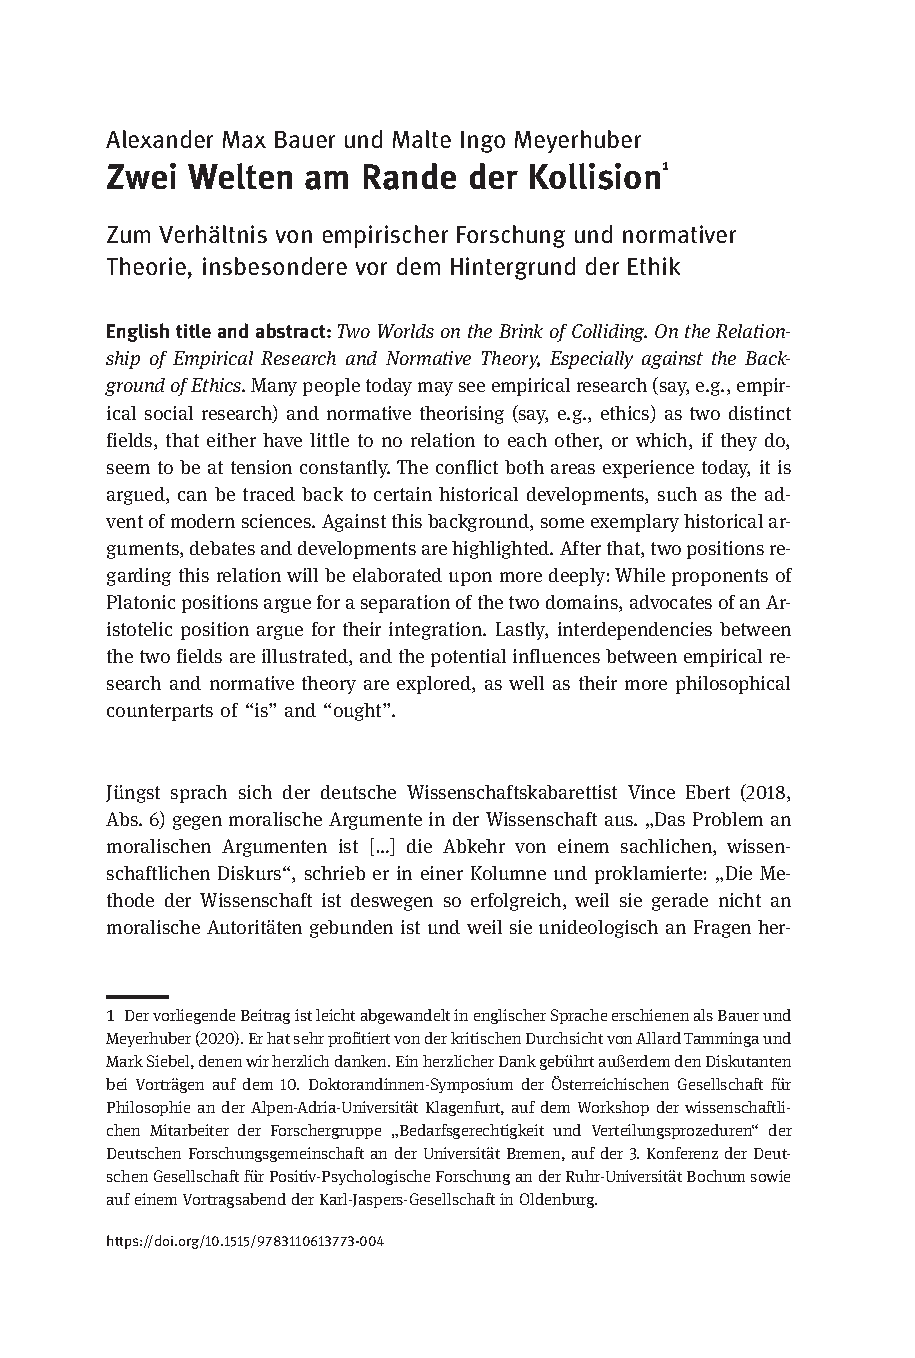
\includegraphics[width=0.6\linewidth]{figures/slides_bauer_meyerhuber_2019.pdf}}\\
      \footnotesize{\textcolor{gray}{Bauer und Meyerhuber 2019}}
   \end{center}
\end{multicols}
\note{
   \begin{itemize}
      \item kein naiver Positivismus
      \item \enquote{platonische} und \enquote{aristotelische} Perspektive \textcolor{gray}{(Miller 1994, S. 177ff.)}
   \end{itemize}
}
\end{frame}


%%%%%%%%%%%%
% FOLIE 10 %
%%%%%%%%%%%%
\begin{frame}
\begin{overlayarea}{\textwidth}{0.81\paperheight}{
   \vspace*{11mm}
   \usebeamerfont{title}\textcolor{uolblue}
   {3\hspace*{1em}Bedarf und Bedarfsgerechtigkeit}
}
\end{overlayarea}
\end{frame}


%%%%%%%%%%%%
% FOLIE 11 %
%%%%%%%%%%%%
\begin{frame}{\vspace*{10mm}3\hspace*{1em}Bedarf und Bedarfsgerechtigkeit}
\begin{multicols}{2}
   \textbf{Gerechtigkeit und Verteilungsgerechtigkeit}\\
   \medskip
   \begin{itemize}
      \item \enquote{So hat [\ldots] Simonides nach Dichterart angedeutet, was das Gerechte sei: daß man jedem gebe, was ihm gebühre, und hat dies als Schuldigkeit bezeichnet} \textcolor{gray}{(Platon 2004, S. 13, 332\,b--c)}
      \item \enquote{Von der Gerechtigkeit im speziellen Sinn und dem in ihrem Sinne Gerechten findet sich die eine Form bei der Verteilung von Ehre, Geld oder anderen Gütern, die unter den Mitgliedern der Staatsgemeinschaft teilbar sind} \textcolor{gray}{(Aristoteles 2011, S. 166, 1130\,b)}
   \end{itemize}
   \vfill
   \begin{center}
      \frame{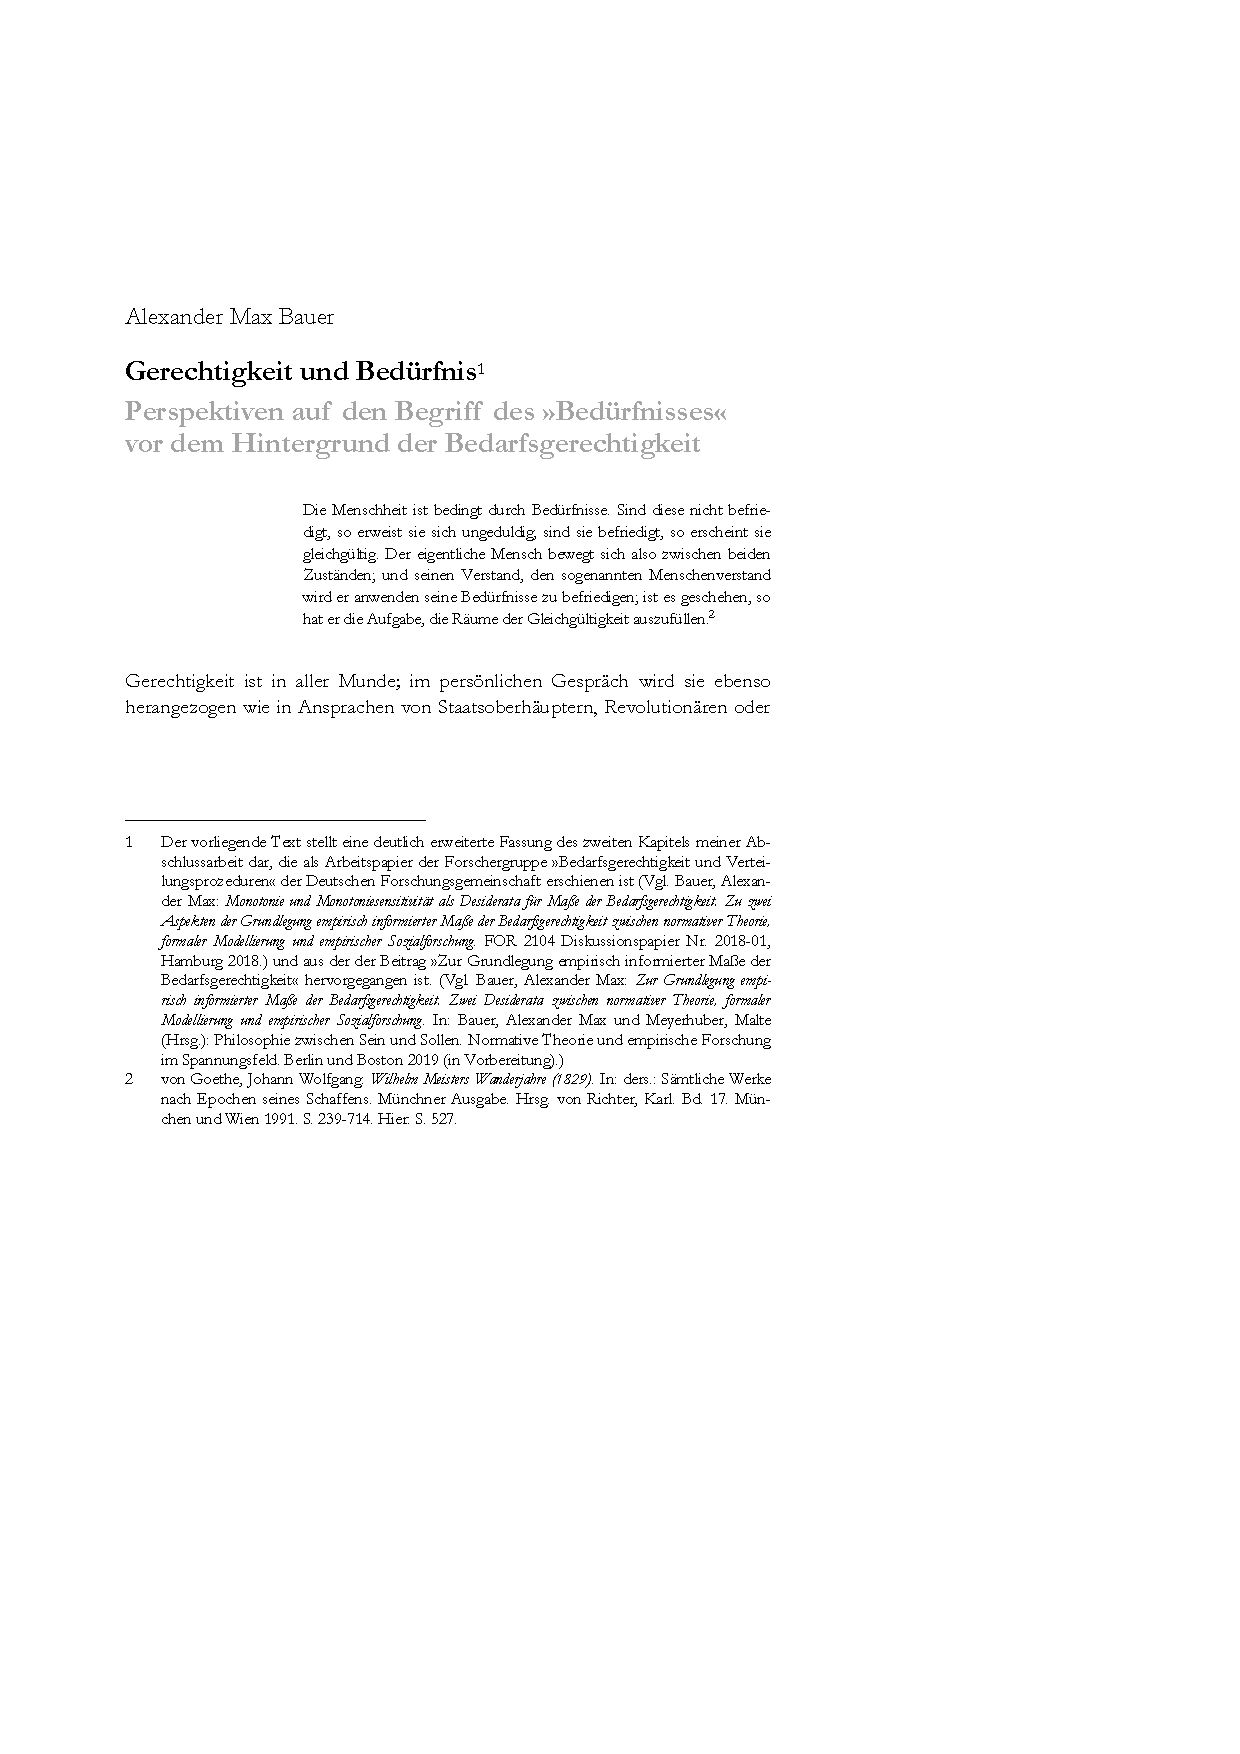
\includegraphics[width=0.6\linewidth]{figures/slides_bauer_2019.pdf}}\\
      \footnotesize{\textcolor{gray}{Bauer 2019}}
   \end{center}
\end{multicols}
\end{frame}


%%%%%%%%%%%%
% FOLIE 12 %
%%%%%%%%%%%%
\begin{frame}{\vspace*{10mm}3\hspace*{1em}Bedarf und Bedarfsgerechtigkeit}
\textbf{Verteilungsprinzipien}\\
\medskip
\enquote{Stellen Sie sich vor, Sie müssten entscheiden, welches der drei Kinder Anne, Bob und Clara die Flöte haben soll, um die sie sich streiten. Anne verlangt das Instrument für sich, da sie als Einzige von den Dreien Flöte spielen könne [\ldots] und da es ungerecht wäre, die Flöte dem einzigen Kind zu verweigern, das tatsächlich auf ihr spielen kann. [\ldots]\\
\medskip
In einem alternativen Szenario meldet sich Bob und verteidigt seinen Anspruch auf die Flöte mit dem Hinweis, er als Einziger von den Dreien sei so arm, dass er keine eigenen Spielzeuge besitze. Bekäme er die Flöte, hätte er etwas zum Spielen. [\ldots]\\
\medskip
In einem zweiten alternativen Szenario kommt Clara zu Wort und erklärt, dass sie viele Monate lang fleißig gearbeitet habe, um die Flöte selbst zu bauen [\ldots].} \textcolor{gray}{(Sen 2012, S. 41)}\\
\begin{center}
   \begin{tikzpicture}
      \draw[very thick,blue2] (15,0) -- (16.1,0.4);
      \draw[very thick,blue2] (15,0) -- (13.9,0.4);
   \end{tikzpicture}\\
   {\color{blue2} \fontsize{10}{10}\selectfont%
   Für sich genommen legitim erscheinende Verteilungsprinzipien\\[0.2ex]
   können miteinander in Konflikt geraten, wenn sie nicht isoliert betrachtet werden}
\end{center}
\note{
   \begin{itemize}
      \item Prinzipienmonismus
      \item Prinzipienpluralismus
      \begin{itemize}
         \item Rangfolge (Rawls)
         \item Kontextabhängigkeit (Walzer)
      \end{itemize}
   \end{itemize}
}
\end{frame}


%%%%%%%%%%%%
% FOLIE 13 %
%%%%%%%%%%%%
\begin{frame}{\vspace*{10mm}3\hspace*{1em}Bedarf und Bedarfsgerechtigkeit}
\textbf{Bedarfsprinzip}\\
\medskip
\begin{itemize}
   \item Verteilungsprinzipien klassifizierbar danach, wer (Umfang) wieviel (Form) wovon (Gut) erhalten soll \textcolor{gray}{(Page 2006, Siebel und Schramme 2020)}
   \item Bedürftige sollen das, dessen sie bedürfen, in vollem Umfang erhalten.
   \begin{itemize}
      \item Wie verteilt man Ressourcen, wenn weniger oder mehr zur Verfügung steht, als insgesamt gebraucht wird?
      \item Wann lässt sich sagen, dass jemand etwas bedarf?
   \end{itemize}
\end{itemize}
\end{frame}


%%%%%%%%%%%%
% FOLIE 14 %
%%%%%%%%%%%%
\begin{frame}{\vspace*{10mm}3\hspace*{1em}Bedarf und Bedarfsgerechtigkeit}
\textbf{Bedarf}\\
\medskip
\begin{itemize}
   \item \textit{S} benötigt \textit{X}, um \textit{Z} in \textit{U} zu erreichen
   \item Unterscheidung zwischen bloß instrumentellen und fundamentalen Bedürfnissen (z.\,B. durch Ermöglichung würdevoller Lebensumstände oder Vermeidung von Schaden)
   \item Abgrenzung von bloßen Präferenzen und Wünschen (z.\,B. durch intersubjektive Anerkennung)
\end{itemize}
\end{frame}


%%%%%%%%%%%%
% FOLIE 15 %
%%%%%%%%%%%%
\begin{frame}
\begin{overlayarea}{\textwidth}{0.81\paperheight}{
   \vspace*{11mm}
   \usebeamerfont{title}\textcolor{uolblue}
   {4\hspace*{1em}Bedarf als Referenzpunkt}
}
\end{overlayarea}
\end{frame}


%%%%%%%%%%%%
% FOLIE 16 %
%%%%%%%%%%%%
\begin{frame}{\vspace*{10mm}4\hspace*{1em}Bedarf als Referenzpunkt}
\begin{multicols}{2}
   \textbf{Hintergrund}\\
   \medskip
   \begin{itemize}
      \item Menschen nehmen graduelle Gerechtigkeitseinschätzungen von Verteilungssituationen vor
      \item Gibt es einen Zusammenhang zwischen Gerechtigkeitseinschätzung und Bedarfsdeckung? Welche Rolle spielt dabei eine Bedarfsschwelle?
   \end{itemize}
   \vfill
   \begin{center}
      \frame{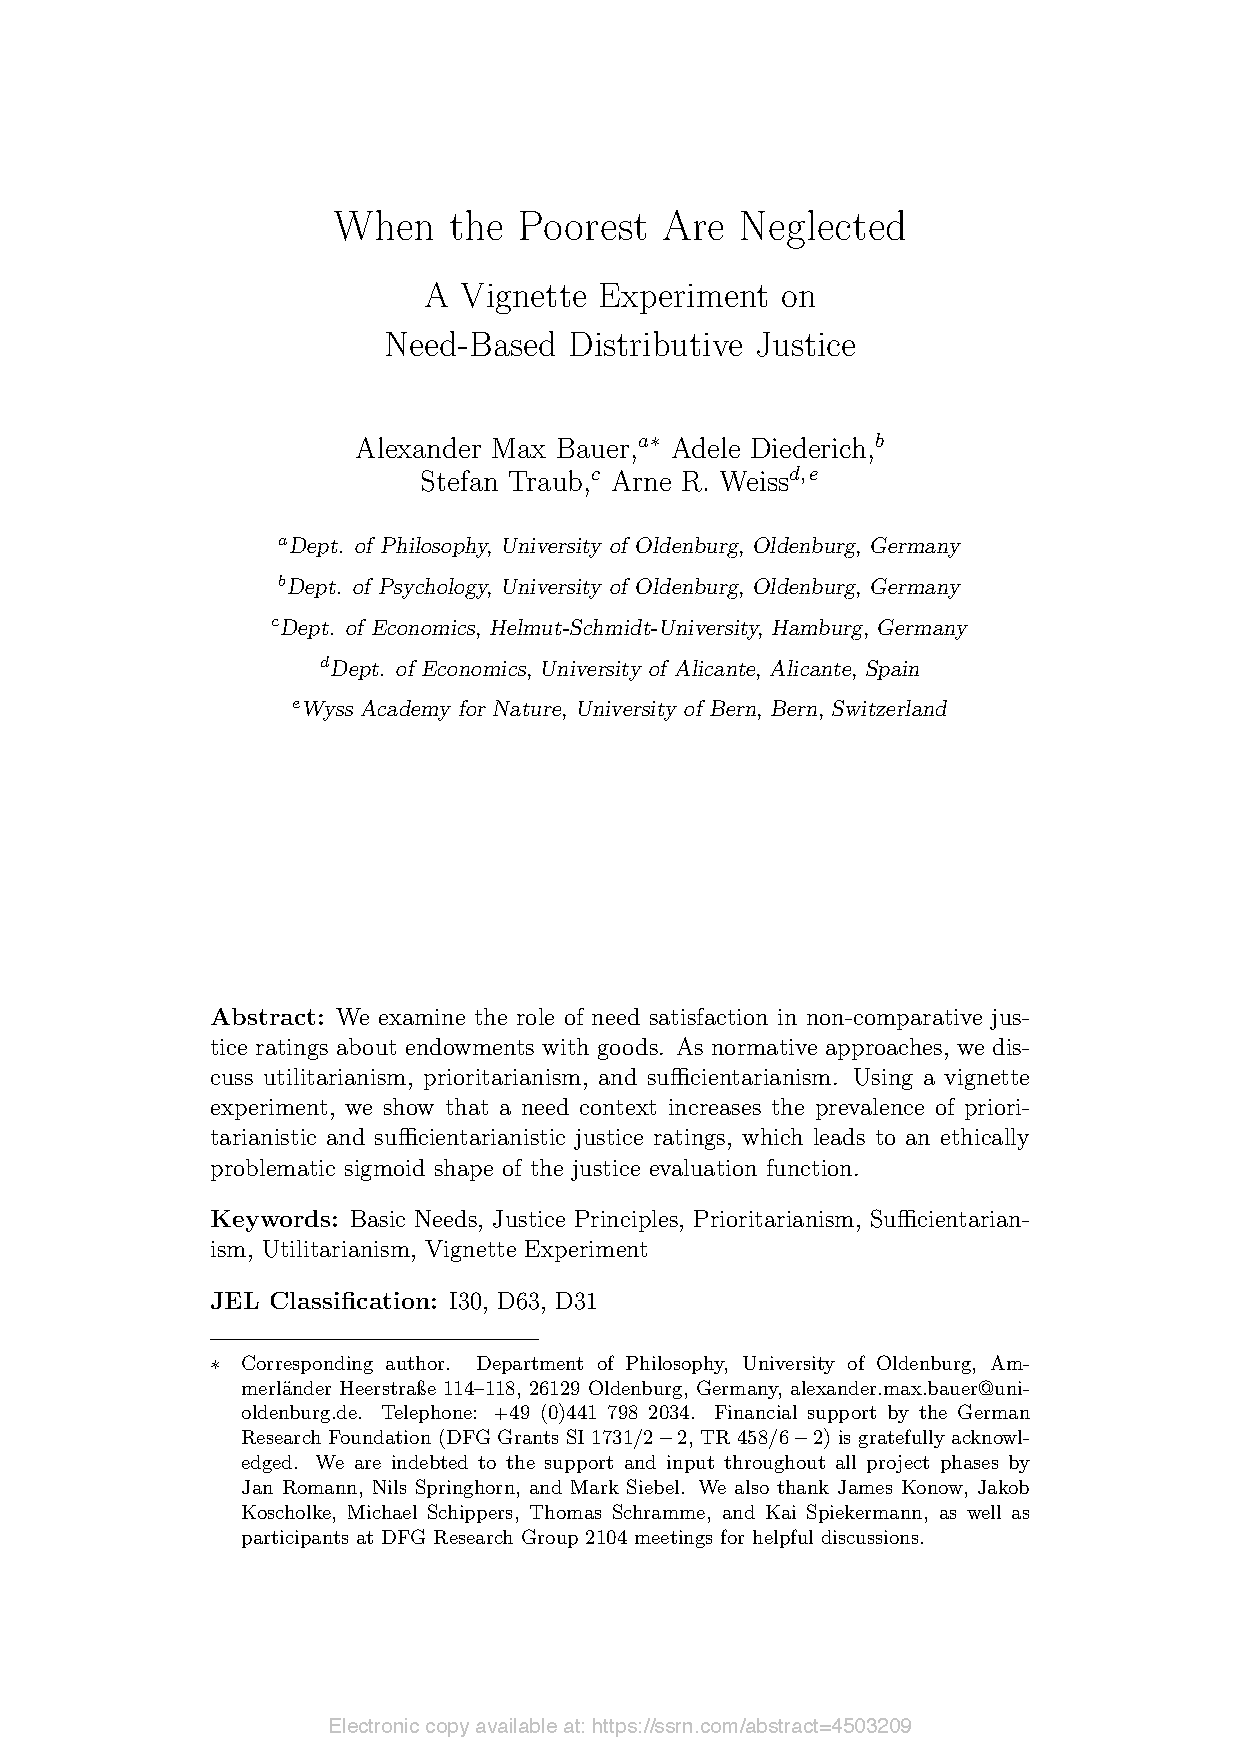
\includegraphics[width=0.6\linewidth]{figures/slides_bauer_et_al_2023a.pdf}}\\
      \footnotesize{\textcolor{gray}{Bauer et al. 2023a}}
   \end{center}
\end{multicols}
\end{frame}


%%%%%%%%%%%%
% FOLIE 17 %
%%%%%%%%%%%%
\begin{frame}{\vspace*{10mm}4\hspace*{1em}Bedarf als Referenzpunkt}
\textbf{Durchführung}\\
\medskip
\begin{itemize}
   \item WiSo-Experimentallabor, Universität Hamburg, 2016
   \item Bedarfs- ($n=52$) und Kontrollgruppe ($n=52$)
   \item $11$ Verteilungssituationen, eingebettet in einen hypothetischen Kontext
   \item Globale und relative Einschätzungsaufgabe
\end{itemize}
\end{frame}


%%%%%%%%%%%%
% FOLIE 18 %
%%%%%%%%%%%%
\begin{frame}{\vspace*{10mm}3\hspace*{1em}Bedarf als Referenzpunkt}
\textbf{Vignette (1/2)}\\
\medskip
\enquote{Bitte stellen Sie sich Folgendes vor:\\
\medskip
In der Region Bergtal soll das neue Dorf Ahdorf gegründet werden. Der dortige Bau von Wohnraum ist Aufgabe der öffentlichen Wohnungsbaugesellschaft von Bergtal.\\
\medskip
Alle Haushalte in dieser Region möchten in möglichst großem Wohnraum leben. Die Bewohner der Region haben sich gemeinsam auf Untergrenzen an Wohnraum verständigt, unterhalb derer ein würdevolles Leben in dieser Gesellschaft nicht möglich ist. Zwischen den Haushalten in dieser Region gibt es keine nennenswerten Unterschiede und die Untergrenzen sind für jeden Haushalt gleich: Jeder Haushalt sollte mindestens über 1.000 regionale -- also in dieser Region gebräuchliche -- Größeneinheiten an Wohnraum verfügen, um ein würdevolles Leben führen zu können. Ein Wohnraum der entsprechenden Größe bedeutet für einen Haushalt zwar ein Leben in beengten Verhältnissen, genügt aber gerade noch, um ein würdevolles Leben führen zu können.}
\end{frame}


%%%%%%%%%%%%
% FOLIE 19 %
%%%%%%%%%%%%
\begin{frame}{\vspace*{10mm}3\hspace*{1em}Bedarf als Referenzpunkt}
\textbf{Vignette (2/2)}\\
\medskip
\enquote{Es sind ausreichend Mittel vorhanden, um für jeden Haushalt bis zu 2.000 regionale Größeneinheiten an Wohnraum bauen zu können. Das Regionalparlament entscheidet, wie viel Wohnraum für die Bewohner des neuen Dorfes tatsächlich gebaut wird. Die Entscheidung hat ansonsten keine nennenswerten Auswirkungen.\\
\medskip
Für den Bau von Wohnraum würde keine zusätzliche Fläche verbraucht. Das neue Dorf soll auf der Fläche eines verlassenen Dorfes gegründet werden, das verlassen wurde, nachdem ein Brand die Häuser zerstört hatte.\\
\medskip
Bei seiner Entscheidung will das Regionalparlament berücksichtigen, wie gerecht die Szenarien von unabhängigen Personen -- wie Ihnen -- beurteilt werden. Ihre Aufgabe ist daher, für jedes Szenario anzugeben, für wie gerecht Sie die Verteilung von Wohnraum jeweils halten.}
\end{frame}


%%%%%%%%%%%%
% FOLIE 20 %
%%%%%%%%%%%%
\begin{frame}{\vspace*{10mm}4\hspace*{1em}Bedarf als Referenzpunkt}
\textbf{Abfrage (1/2)}\\
\bigskip
\begin{center}
   \frame{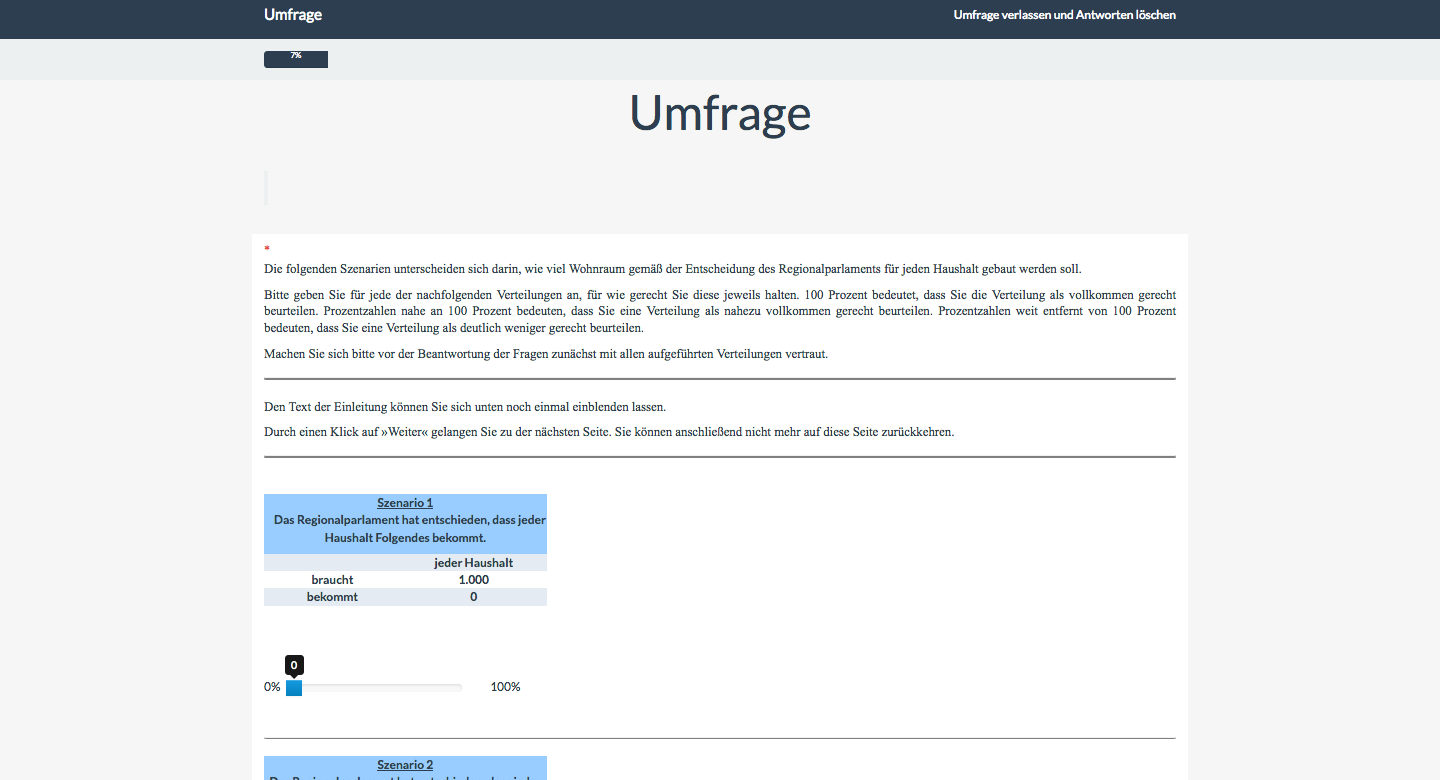
\includegraphics[width=0.5\linewidth]{figures/slides_lime_1.png}}\\
   \footnotesize{\textcolor{gray}{Globale Einschätzungsaufgabe}}
\end{center}
\end{frame}


%%%%%%%%%%%%
% FOLIE 21 %
%%%%%%%%%%%%
\begin{frame}{\vspace*{10mm}4\hspace*{1em}Bedarf als Referenzpunkt}
\textbf{Abfrage (2/2)}\\
\begin{multicols}{2}
   \begin{center}
      \frame{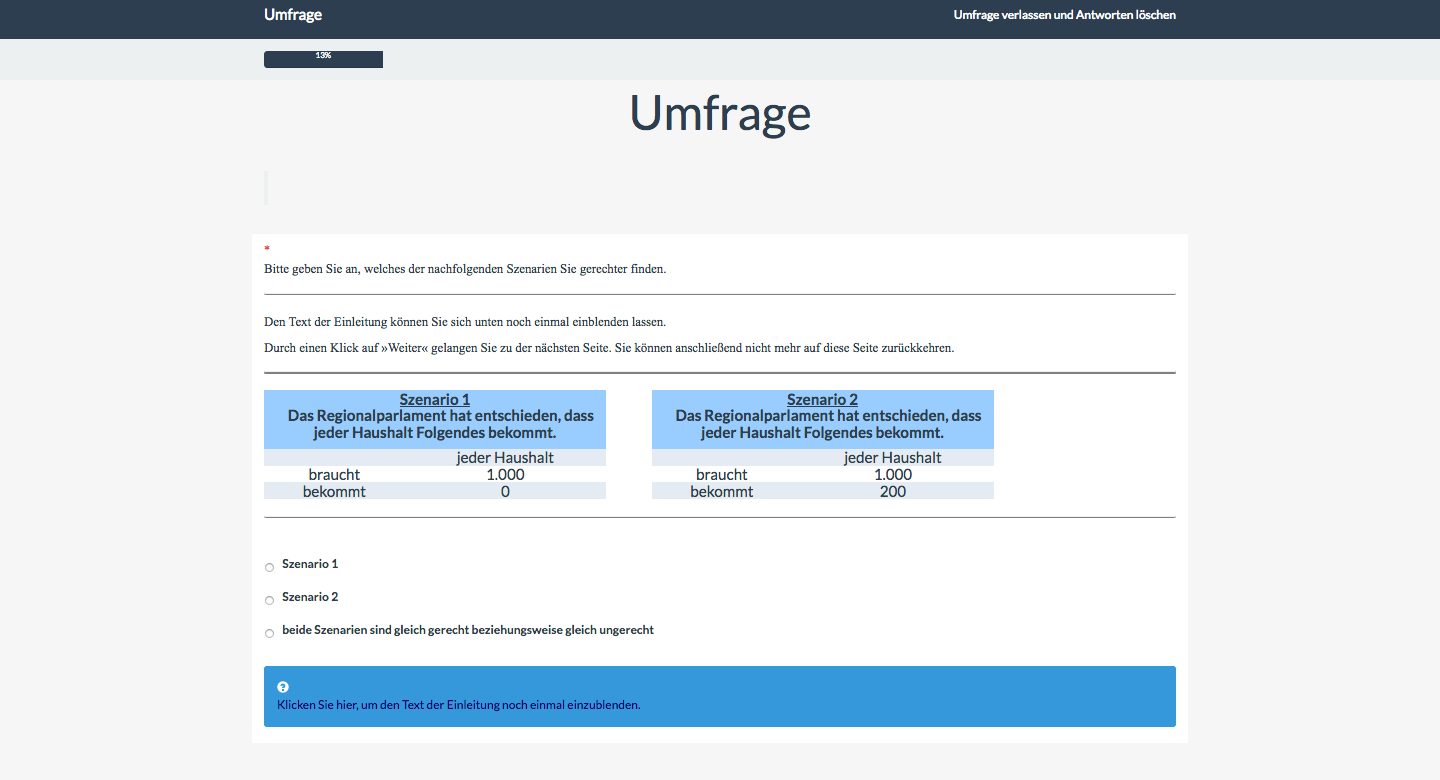
\includegraphics[width=1\linewidth]{figures/slides_lime_2.png}}\\
      \footnotesize{\textcolor{gray}{Relative Einschätzungsaufgabe, Teil 1}}
      \frame{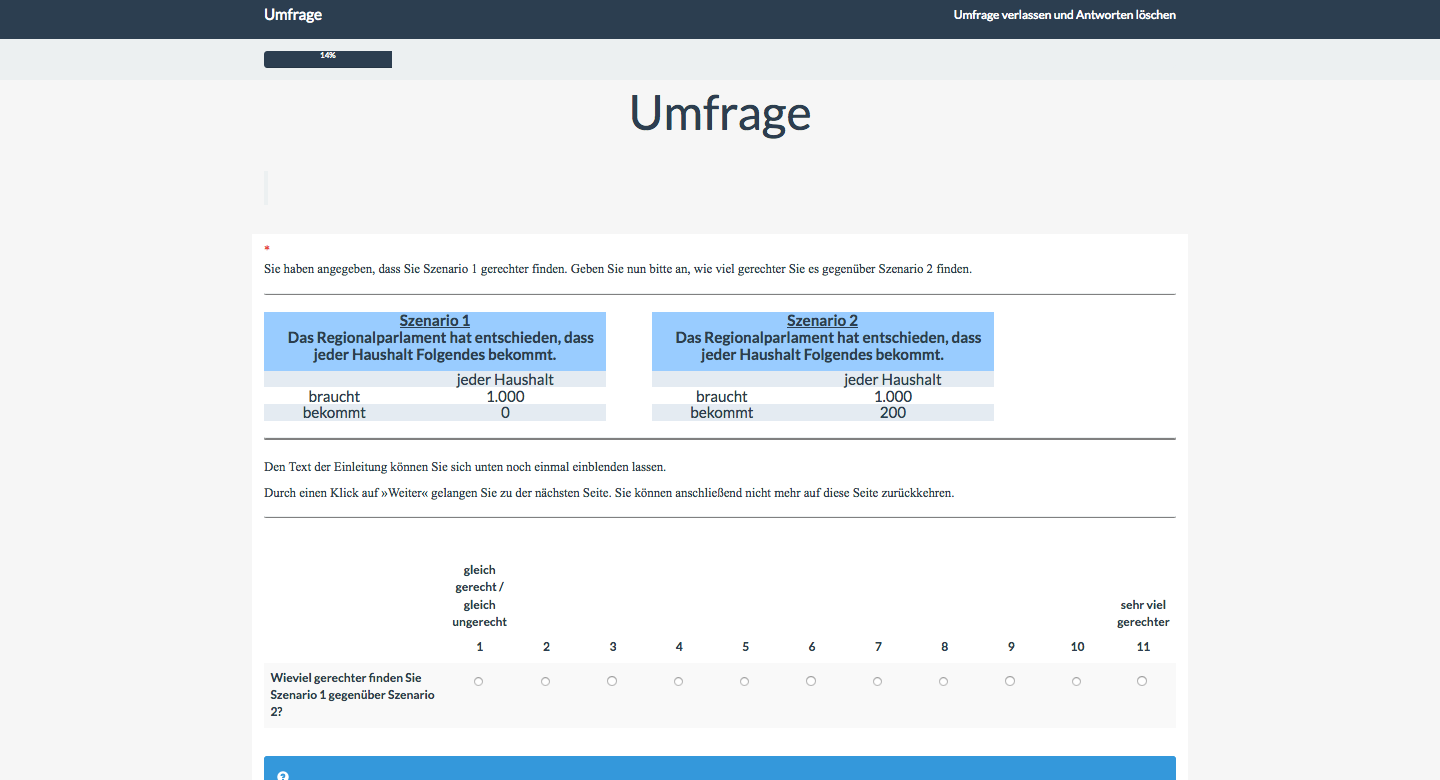
\includegraphics[width=1\linewidth]{figures/slides_lime_3.png}}\\
      \footnotesize{\textcolor{gray}{Relative Einschätzungsaufgabe, Teil 2}}
   \end{center}
\end{multicols}
\end{frame}


%%%%%%%%%%%%
% FOLIE 22 %
%%%%%%%%%%%%
\begin{frame}{\vspace*{10mm}4\hspace*{1em}Bedarf als Referenzpunkt}
\textbf{Ergebnisse (1/2)}\\
\medskip
\begin{multicols}{2}
   \begin{center}
      \frame{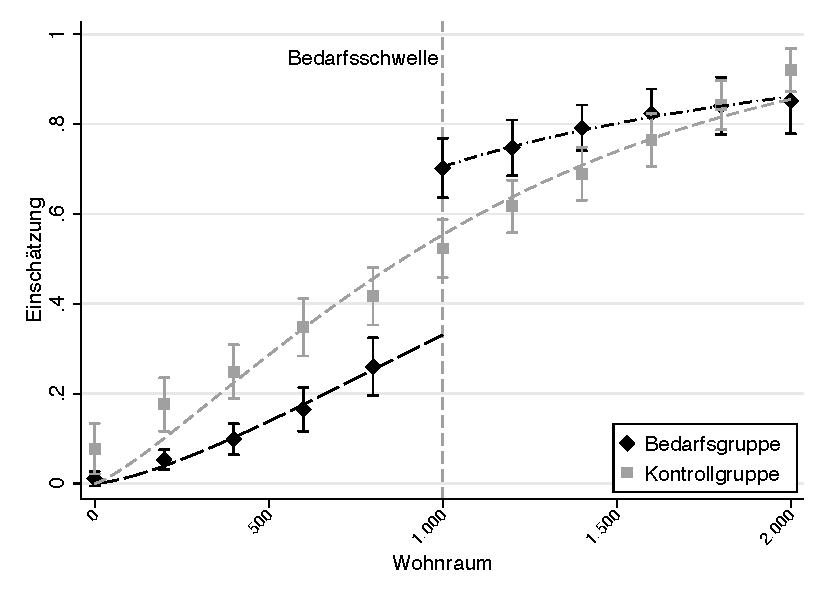
\includegraphics[width=1\linewidth]{figures/figure_1.pdf}}\\
      \footnotesize{\textcolor{gray}{Globale Einschätzungsaufgabe}}
      \frame{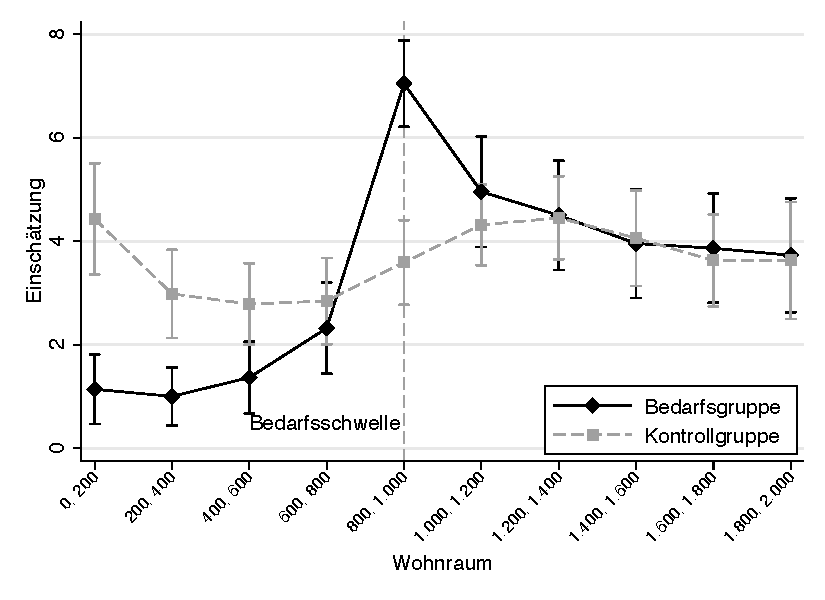
\includegraphics[width=1\linewidth]{figures/figure_2.pdf}}\\
      \footnotesize{\textcolor{gray}{Relative Einschätzungsaufgabe}}
   \end{center}
\end{multicols}
\note{
   \begin{itemize}
      \item Globale Einschätzungsaufgabe
      \begin{itemize}
         \item Weibul-Schätzung (Referenzpunkte bei 0 und 1.000 Einheiten)
         \item Sprunghafter Anstieg (etwa 35 Prozentpunkte), unterhalb der Schwelle konvex, oberhalb konkav
         \item Einschätzungen unterhalb der Schwelle (mit Ausnahme von 0 Einheiten) in Bedarfsgruppe signifikant niedriger
         \item Einschätzungen oberhalb der Schwelle (mit Ausnahme von 1.600, 1,800 und 2.000 Einheiten) in Bedarfsgruppe signifikant höher
      \end{itemize}
      \item Relative Einschätzungsaufgabe
      \begin{itemize}
         \item Vergleiche in Kontrollgruppe mäandern um 3 und 4 Punkte
         \item Lorem ipsum...
      \end{itemize}
   \end{itemize}
}

\end{frame}


%%%%%%%%%%%%
% FOLIE 23 %
%%%%%%%%%%%%
\begin{frame}{\vspace*{10mm}4\hspace*{1em}Bedarf als Referenzpunkt}
\textbf{Ergebnisse (2/2)}\\
\medskip
\begin{itemize}
   \item Unparteiische Beobachter*innen nehmen graduelle Gerechtigkeitseinschätzungen vor
   \item Einschätzungen abhängig von Versorgungssituationen
   \item Bedarfsinformationen beeinflussen Einschätzungen
\end{itemize}
\end{frame}


%%%%%%%%%%%%
% FOLIE 24 %
%%%%%%%%%%%%
\begin{frame}
\begin{overlayarea}{\textwidth}{0.81\paperheight}{
   \vspace*{11mm}
   \usebeamerfont{title}\textcolor{uolblue}
   {5\hspace*{1em}Bedarf und Verantwortung}
}
\end{overlayarea}
\end{frame}


%%%%%%%%%%%%
% FOLIE 25 %
%%%%%%%%%%%%
\begin{frame}{\vspace*{10mm}5\hspace*{1em}Bedarf und Verantwortung}
\begin{multicols}{2}
   \begin{itemize}
      \item Lorem
      \item Ipsum
      \item Dolor
   \end{itemize}
   \vfill
   \begin{center}
      \frame{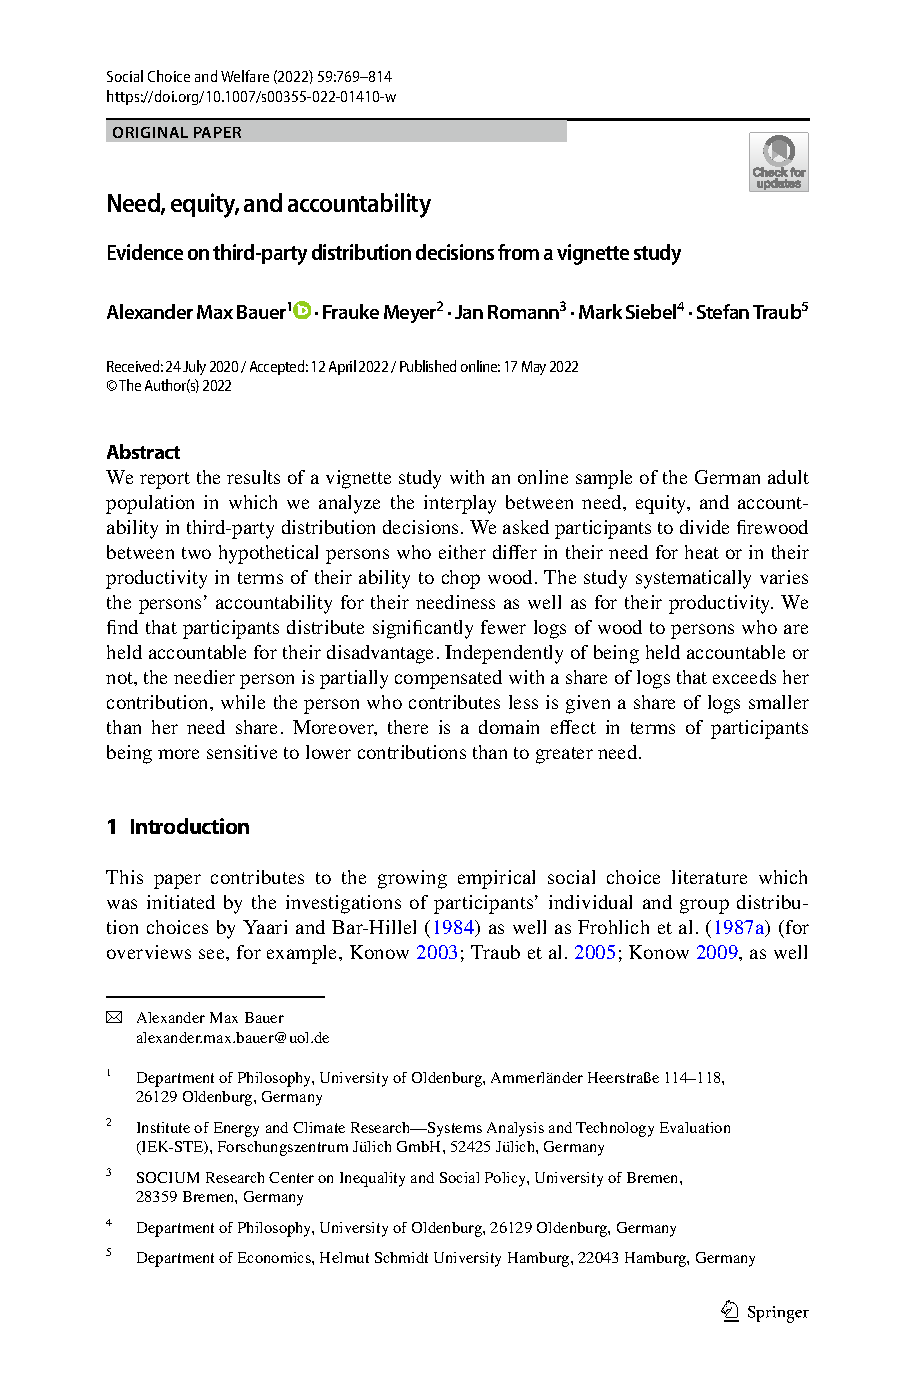
\includegraphics[width=0.6\linewidth]{figures/slides_bauer_et_al_2022.pdf}}\\
      \footnotesize{\textcolor{gray}{Bauer et al. 2022}}
   \end{center}
\end{multicols}
\end{frame}


%%%%%%%%%%%%
% FOLIE 26 %
%%%%%%%%%%%%
\begin{frame}
\begin{overlayarea}{\textwidth}{0.81\paperheight}{
   \vspace*{11mm}
   \usebeamerfont{title}\textcolor{uolblue}
   {6\hspace*{1em}Bedarfsarten}
}
\end{overlayarea}
\end{frame}


%%%%%%%%%%%%
% FOLIE 27 %
%%%%%%%%%%%%
\begin{frame}{\vspace*{10mm}6\hspace*{1em}Bedarfsarten}
\begin{multicols}{2}
   \begin{itemize}
      \item Lorem
      \item Ipsum
      \item Dolor
   \end{itemize}
   \vfill
   \begin{center}
      \frame{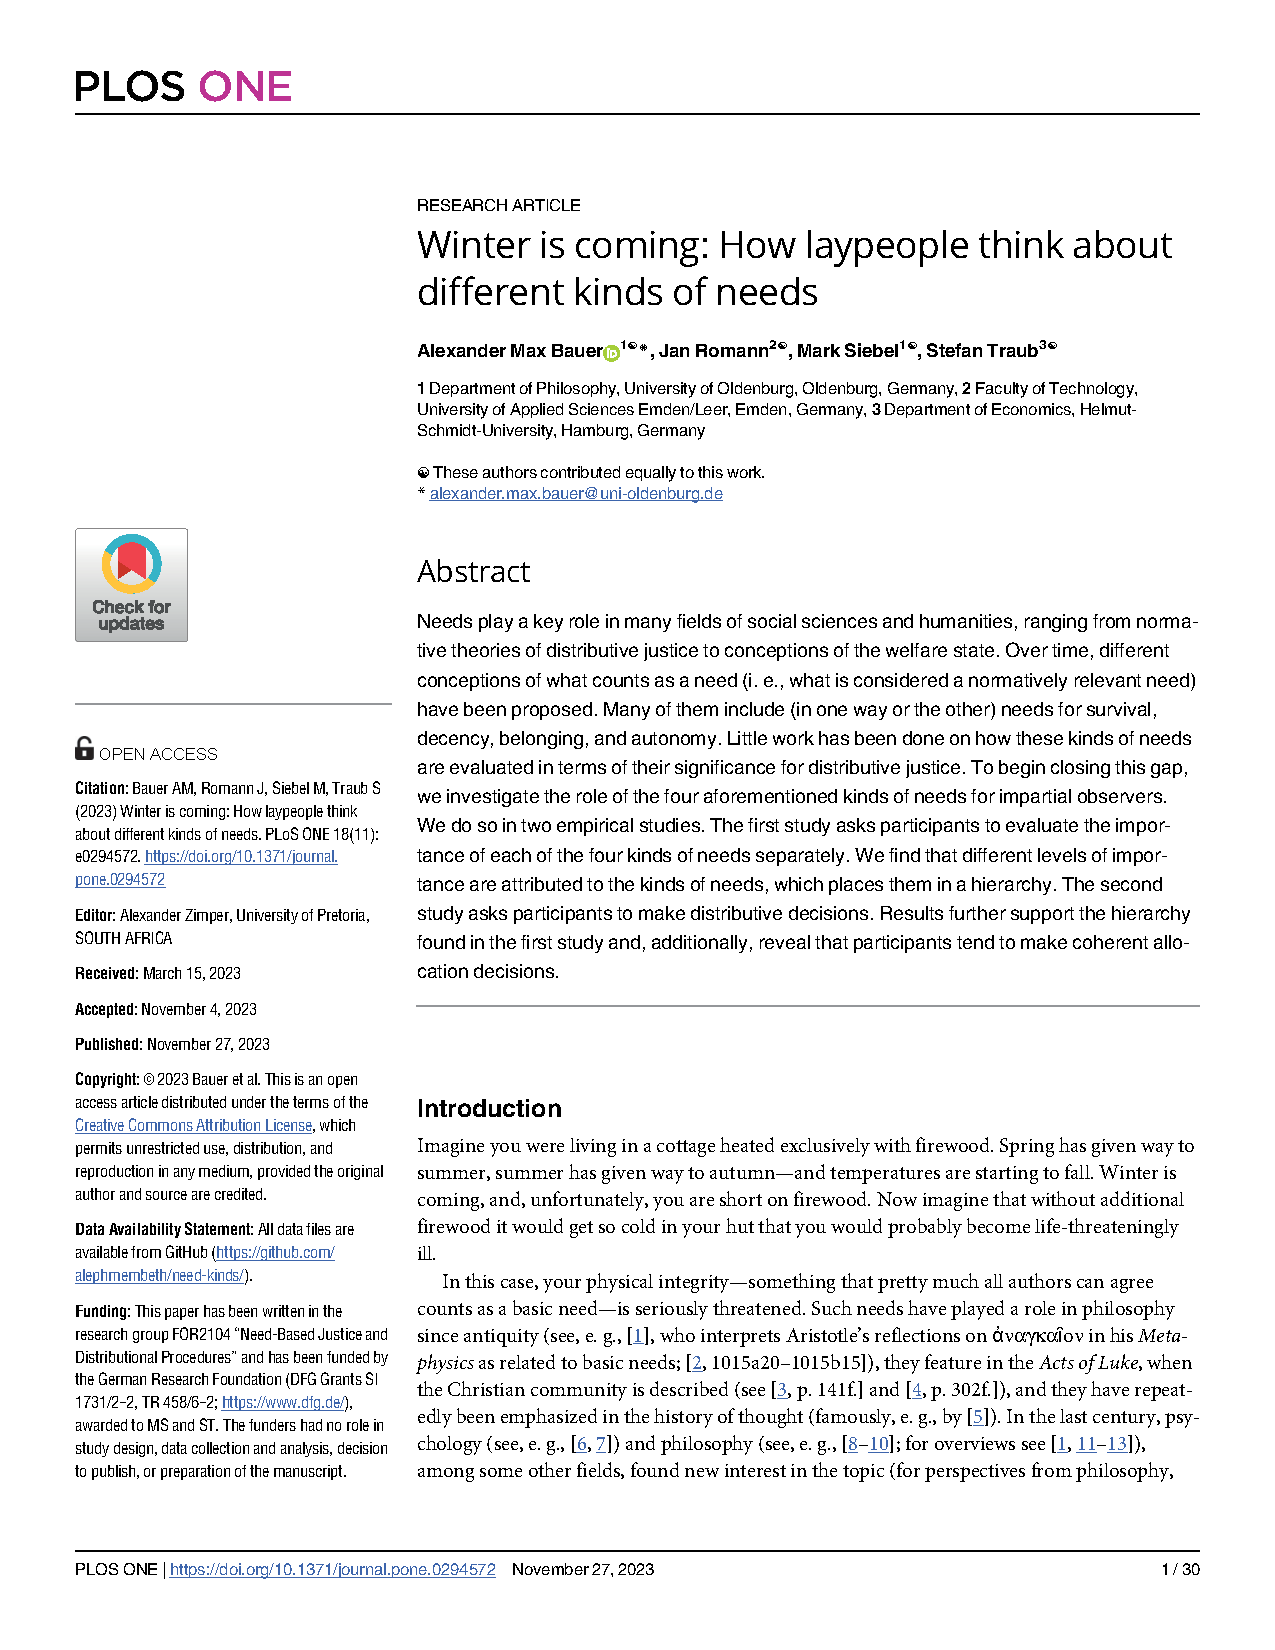
\includegraphics[width=0.6\linewidth]{figures/slides_bauer_et_al_2023b.pdf}}\\
      \footnotesize{\textcolor{gray}{Bauer et al. 2023b}}
   \end{center}
\end{multicols}
\end{frame}


%%%%%%%%%%%%
% FOLIE 28 %
%%%%%%%%%%%%
\begin{frame}
\begin{overlayarea}{\textwidth}{0.81\paperheight}{
   \vspace*{11mm}
   \usebeamerfont{title}\textcolor{uolblue}
   {7\hspace*{1em}Zusammenfassung\\\hspace*{1.5em}zentraler Ergebnisse}
}
\end{overlayarea}
\end{frame}


%%%%%%%%%%%%
% FOLIE 29 %
%%%%%%%%%%%%
\begin{frame}{\vspace*{10mm}7\hspace*{1em}Zusammenfassung zentraler Ergebnisse}
\vspace*{-10mm}
\begin{itemize}
   \item[(1)] Unparteiische Beobachter*innen nehmen graduelle Gerechtigkeitseinschätzungen vor
   \item[(2)] Diese Einschätzungen sind abhängig von Versorgungssituationen
   \item[(3)] Bedarfsinformationen beeinflussen diese Einschätzungen
\end{itemize}
\vspace{1em}
\begin{itemize}
   \item[(4)] Unparteiische Entscheider*innen berücksichtigen Bedarf, Leistung und Verantwortung
   \item[(5)] Auch bei zu geringer Leistung wird Bedarf teilweise kompensiert
   \item[(6)] Kompensationsbereitschaft sinkt, wenn zu geringe Leistung selbst verschuldet ist
\end{itemize}
\vspace{1em}
\begin{itemize}
   \item[(7)] Unparteiische Beobachter*innen und Entscheider*innen unterscheiden Bedarfsarten
\end{itemize}
\end{frame}


%%%%%%%%%%%%
% FOLIE 30 %
%%%%%%%%%%%%
\begin{frame}{}
\begin{center}
   
\includegraphics[width=0.8\linewidth]{figures/slides_thanks.pdf}
\end{center}
\end{frame}


%%%%%%%%%%%%
% FOLIE 31 %
%%%%%%%%%%%%
\begin{frame}{\vspace*{10mm}Bibliografie}
\vspace*{-10mm}
{\footnotesize
\begin{itemize}[label=,leftmargin=2em,itemindent=-2em]
   \item Aristoteles (2011): \textit{Nikomachische Ethik}. Hrsg. von Ursula Wolf. Hamburg: Rowohlt.
   \item Bauer, Alexander Max (2019): \enquote{Gerechtigkeit und Bedürfnis. Perspektiven auf den Begriff des \enquote{Bedürfnisses} vor dem Hintergrund der Bedarfsgerechtigkeit}. In: Alexander Max Bauer und Nils Baratella (Hrsg.): \textit{Oldenburger Jahrbuch für Philosophie 2017/2018}. Oldenburg: BIS-Verlag. S. 285--327.
   \item Bauer, Alexander Max, Adele Diederich, Stefan Traub und Arne Robert Weiss (2023): \enquote{When the Poorest Are Neglected. A Vignette Experiment on Need-Based Distributive Justice}. \textit{SSRN Working Paper} 4503209.
   \item Bauer, Alexander Max, Frauke Meyer, Jan Romann, Mark Siebel und Stefan Traub (2022): \enquote{Need, Equity, and Accountability. Evidence on Third-Party Distributive Decisions from a Vignette Study}. In: \textit{Social Choice and Welfare} 59, S. 769--814.
   \item Bauer, Alexander Max und Malte Ingo Meyerhuber (2019): \enquote{Zwei Welten am Rande der Kollision. Zum Verhältnis von empirischer Forschung und normativer Theorie, insbesondere vor dem Hintergrund der Ethik}. In: dies. (Hrsg.): \textit{Philosophie zwischen Sein und Sollen. Normative Theorie und empirische Forschung im Spannungsfeld}. Berlin und Boston: Walter de Gruyter. S. 13--37.
\end{itemize}
}
\end{frame}


%%%%%%%%%%%%
% FOLIE 32 %
%%%%%%%%%%%%
\begin{frame}{\vspace*{10mm}Bibliografie}
\vspace*{-10mm}
{\footnotesize
\begin{itemize}[label=,leftmargin=2em,itemindent=-2em]
   \item Bauer, Alexander Max und Jan Romann (i.\,V.): \enquote{Equal Deeds, Different Needs. Need, Accountability, and Ressource Availability in Third-Party Distributive Decisions}. In: Shaun Nichols und Joshua Knobe (Hrsg.): \textit{Oxford Studies in Experimental Philosophy}. Oxford: Oxford University Press.
   \item Bauer, Alexander Max, Jan Romann, Mark Siebel und Stefan Traub (2023): \enquote{Winter is Coming. How Laypeople Think About Different Kinds of Needs}. \textit{PLoS ONE} 18 (11), e0294572.
   \item Bauer, Alexander Max und Mark Siebel (i.\,V.): \enquote{Measuring Need-Based Distributive Justice -- Formally and Empirically}. In: Stefan Traub und Bernhard Kittel (Hrsg.): \textit{Priority of Needs. An Informed Theory of Need-Based Justice}. Cham: Springer.
   \item Platon (2004): \enquote{Der Staat}. In: ders.: \textit{Sämtliche Werke in drei Bänden}. Bd. 2. Hrsg. von Erich Loewenthal. Übers. von Wilhelm Sigismund Teuffel und Wilhelm Wiegand. Darmstadt: Wissenschaftliche Buchgesellschaft. S. 5--407.
   \item Sen, Amartya (2012): \textit{Die Idee der Gerechtigkeit}. München: Deutscher Taschenbuch Verlag.
\end{itemize}
}
\end{frame}


%%%%%%%%%%%%
% FOLIE 33 %
%%%%%%%%%%%%
\begin{frame}
\begin{overlayarea}{\textwidth}{0.81\paperheight}
   {
   \vspace*{11mm}
   \usebeamerfont{title}\textcolor{uolblue}
   {Zusätzliche Folien}
   }
\end{overlayarea}
\end{frame}


%%%%%%%%%%%%
% FOLIE 34 %
%%%%%%%%%%%%
\begin{frame}{\vspace*{10mm}2\hspace*{1em}Empirische Forschung und normative Theorie}
\begin{center}
   \frame{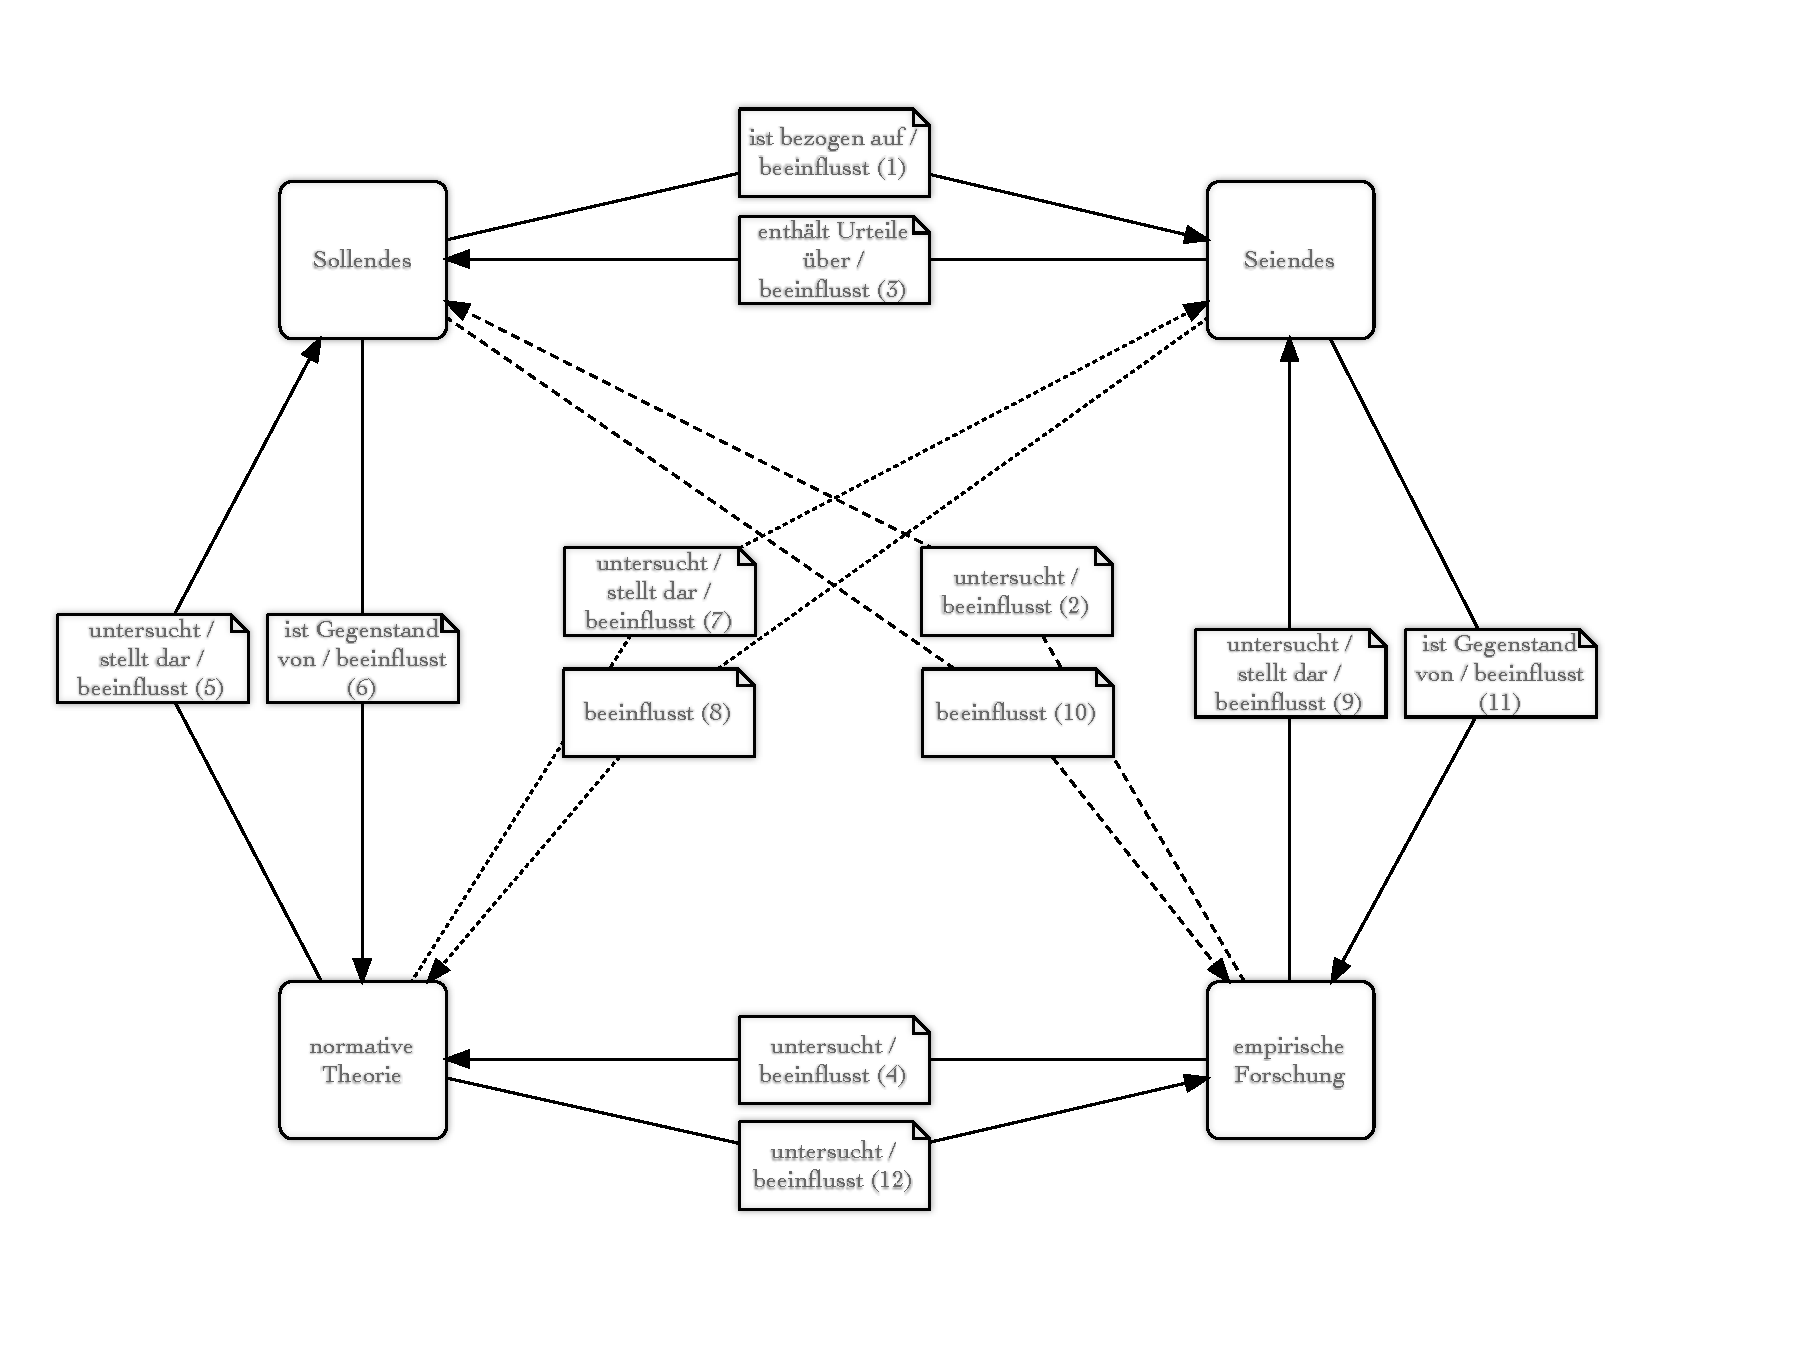
\includegraphics[width=0.6\linewidth]{figures/slides_emp_norm.pdf}}\\
   \footnotesize{\textcolor{gray}{Bauer und Meyerhuber 2019, S. 26}}
\end{center}
\end{frame}


%%%%%%%%%%%%
% FOLIE 35 %
%%%%%%%%%%%%
\begin{frame}{\vspace*{10mm}3\hspace*{1em}Bedarf und Bedarfsgerechtigkeit}
\begin{center}
   \frame{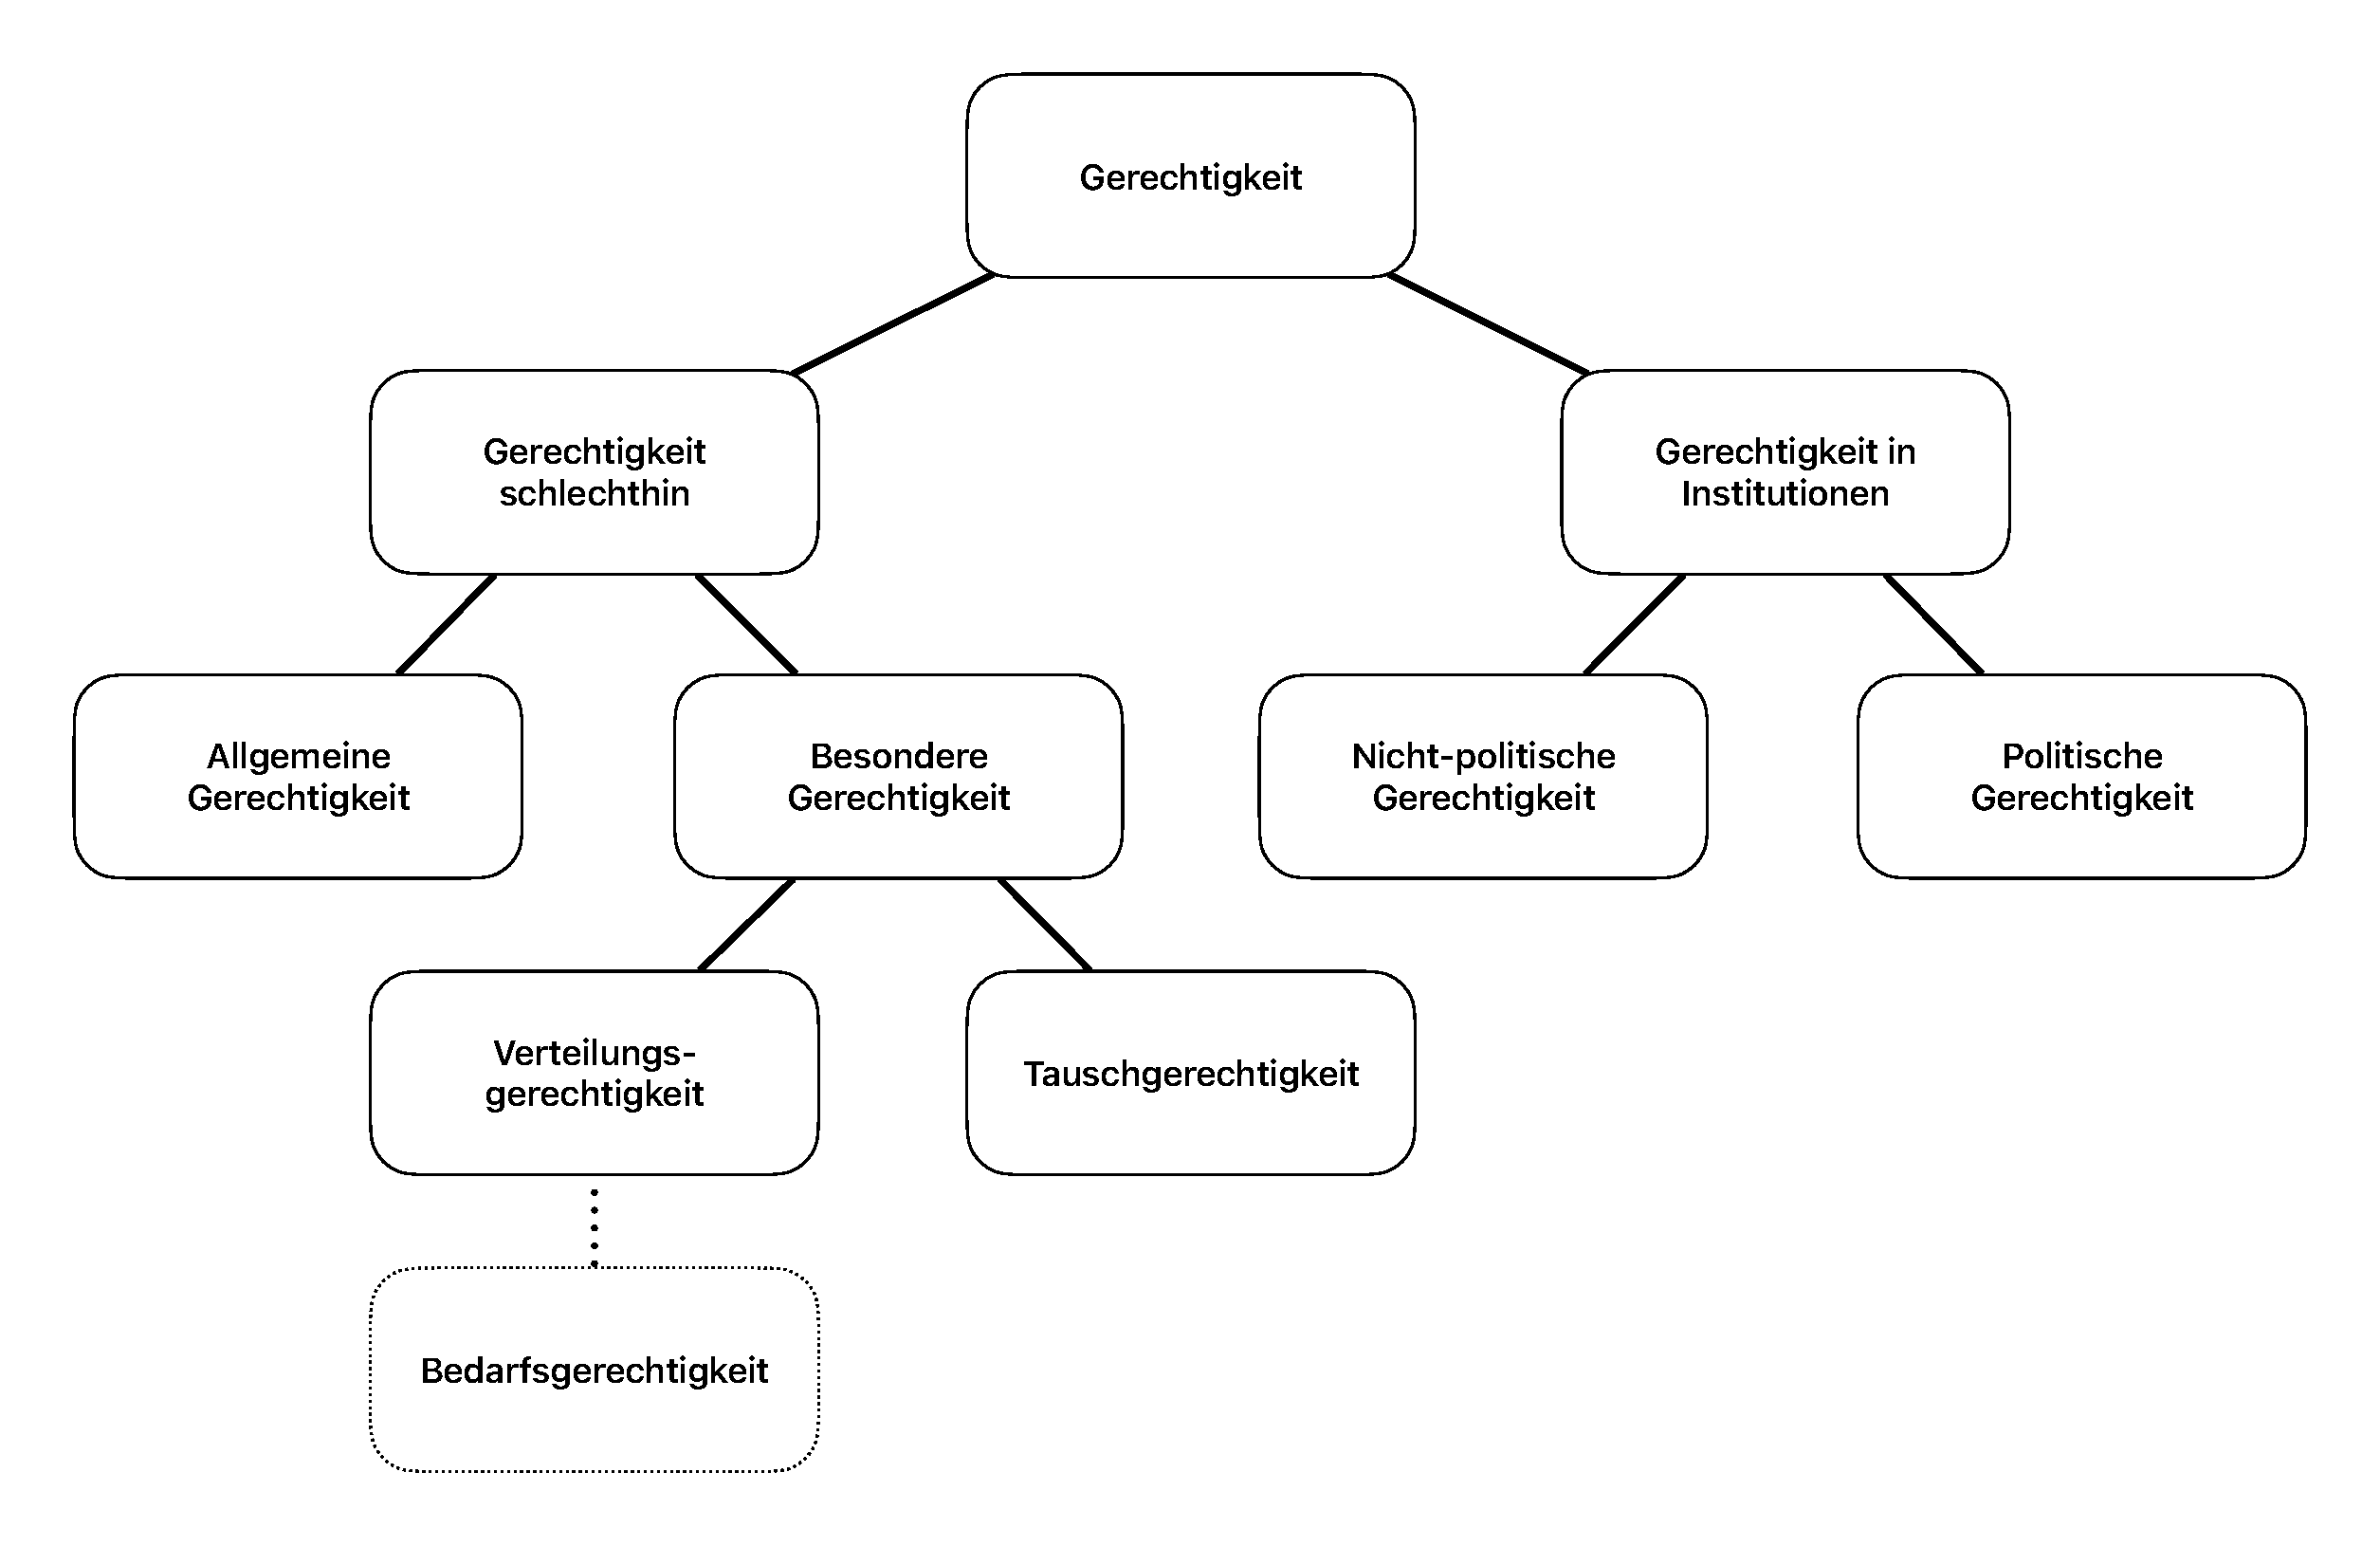
\includegraphics[width=0.7\linewidth]{figures/slides_justice.pdf}}
\end{center}
\end{frame}


%%%%%%%%%%%%
% FOLIE 36 %
%%%%%%%%%%%%
\begin{frame}{\vspace*{10mm}4\hspace*{1em}Bedarf als Referenzpunkt}
\begin{multicols}{2}
   \begin{center}
      \frame{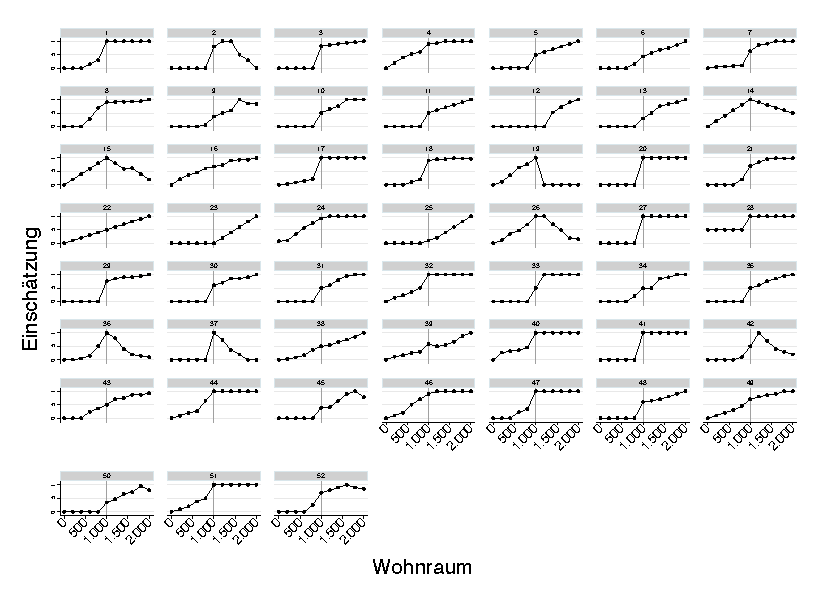
\includegraphics[width=1\linewidth]{figures/figure_3.pdf}}\\
      \footnotesize{\textcolor{gray}{Bedarfsgruppe}}
      \frame{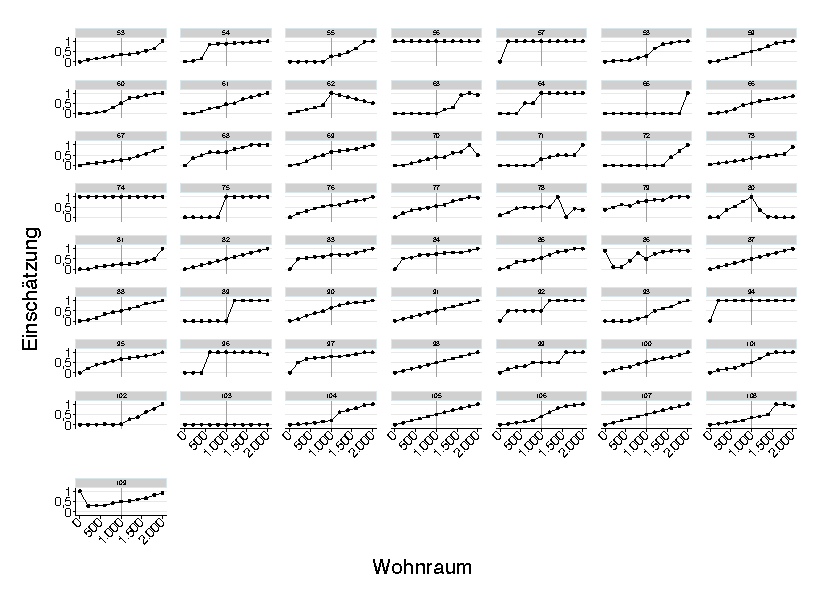
\includegraphics[width=1\linewidth]{figures/figure_4.pdf}}\\
      \footnotesize{\textcolor{gray}{Kontrollgruppe}}
   \end{center}
\end{multicols}
\end{frame}


%%%%%%%%%%%%
% FOLIE 37 %
%%%%%%%%%%%%
\begin{frame}{\vspace*{10mm}4\hspace*{1em}Bedarf als Referenzpunkt}
\begin{center}
   \begin{tabular}[h]{lrrrrrrl}
      \arrayrulecolor{blue2}
      \hline
      Typ              & \multicolumn{5}{c}{Häufigkeit}      &   & Prinzip                                                              \\
      \cline{2-6}
                       & \multicolumn{2}{c}{Bedarfsgruppe}   &   & \multicolumn{2}{c}{Kontrollgruppe}   &   &                           \\
      \hline
      Hügelförmig      &  8   &  (15,38\,\%)                 &   &  2   &   (3,51\,\%)                  &   & \enquote{Strikter}        \\
                       &      &                              &   &      &                               &   & Suffizientarismus         \\[1ex]
      Binär            &  4   &   (7,69\,\%)                 &   &  5   &   (8,77\,\%)                  &   & \enquote{Qualitativer}    \\
                       &      &                              &   &      &                               &   & Suffizientarismus         \\[1ex]
      Flach ab         &  7   &  (13,46\,\%)                 &   &  1   &   (1,75\,\%)                  &   & \enquote{Quantitativer}   \\
      der Schwelle     &      &                              &   &      &                               &   & Suffizientarismus         \\[1ex]
      Null unterhalb   & 15   &  (28,85\,\%)                 &   &  5   &   (8,77\,\%)                  &   & \enquote{Strikter}        \\
      der Schwelle     &      &                              &   &      &                               &   & Prioritarismus            \\[1ex]
      Ansteigend       & 17   &  (32,69\,\%)                 &   & 36   &  (63,16\,\%)                  &   & Utilitarismus             \\[1ex]
      Anderes          &  1   &   (1,92\,\%)                 &   &  8   &  (14,04\,\%)                  &   &                           \\
      \hline
                       & 52   & (100,00\,\%)                 &   & 57   & (100,00\,\%)                  &   &                           \\
      \hline
   \end{tabular}\\
   \smallskip
   \footnotesize{\textcolor{gray}{Einschätzungstypen}}
\end{center}
\end{frame}


\end{document}
